% Options for packages loaded elsewhere
% Options for packages loaded elsewhere
\PassOptionsToPackage{unicode}{hyperref}
\PassOptionsToPackage{hyphens}{url}
\PassOptionsToPackage{dvipsnames,svgnames,x11names}{xcolor}
%
\documentclass[
  letterpaper,
  DIV=11,
  numbers=noendperiod]{scrreprt}
\usepackage{xcolor}
\usepackage{amsmath,amssymb}
\setcounter{secnumdepth}{5}
\usepackage{iftex}
\ifPDFTeX
  \usepackage[T1]{fontenc}
  \usepackage[utf8]{inputenc}
  \usepackage{textcomp} % provide euro and other symbols
\else % if luatex or xetex
  \usepackage{unicode-math} % this also loads fontspec
  \defaultfontfeatures{Scale=MatchLowercase}
  \defaultfontfeatures[\rmfamily]{Ligatures=TeX,Scale=1}
\fi
\usepackage{lmodern}
\ifPDFTeX\else
  % xetex/luatex font selection
\fi
% Use upquote if available, for straight quotes in verbatim environments
\IfFileExists{upquote.sty}{\usepackage{upquote}}{}
\IfFileExists{microtype.sty}{% use microtype if available
  \usepackage[]{microtype}
  \UseMicrotypeSet[protrusion]{basicmath} % disable protrusion for tt fonts
}{}
\makeatletter
\@ifundefined{KOMAClassName}{% if non-KOMA class
  \IfFileExists{parskip.sty}{%
    \usepackage{parskip}
  }{% else
    \setlength{\parindent}{0pt}
    \setlength{\parskip}{6pt plus 2pt minus 1pt}}
}{% if KOMA class
  \KOMAoptions{parskip=half}}
\makeatother
% Make \paragraph and \subparagraph free-standing
\makeatletter
\ifx\paragraph\undefined\else
  \let\oldparagraph\paragraph
  \renewcommand{\paragraph}{
    \@ifstar
      \xxxParagraphStar
      \xxxParagraphNoStar
  }
  \newcommand{\xxxParagraphStar}[1]{\oldparagraph*{#1}\mbox{}}
  \newcommand{\xxxParagraphNoStar}[1]{\oldparagraph{#1}\mbox{}}
\fi
\ifx\subparagraph\undefined\else
  \let\oldsubparagraph\subparagraph
  \renewcommand{\subparagraph}{
    \@ifstar
      \xxxSubParagraphStar
      \xxxSubParagraphNoStar
  }
  \newcommand{\xxxSubParagraphStar}[1]{\oldsubparagraph*{#1}\mbox{}}
  \newcommand{\xxxSubParagraphNoStar}[1]{\oldsubparagraph{#1}\mbox{}}
\fi
\makeatother

\usepackage{color}
\usepackage{fancyvrb}
\newcommand{\VerbBar}{|}
\newcommand{\VERB}{\Verb[commandchars=\\\{\}]}
\DefineVerbatimEnvironment{Highlighting}{Verbatim}{commandchars=\\\{\}}
% Add ',fontsize=\small' for more characters per line
\usepackage{framed}
\definecolor{shadecolor}{RGB}{241,243,245}
\newenvironment{Shaded}{\begin{snugshade}}{\end{snugshade}}
\newcommand{\AlertTok}[1]{\textcolor[rgb]{0.68,0.00,0.00}{#1}}
\newcommand{\AnnotationTok}[1]{\textcolor[rgb]{0.37,0.37,0.37}{#1}}
\newcommand{\AttributeTok}[1]{\textcolor[rgb]{0.40,0.45,0.13}{#1}}
\newcommand{\BaseNTok}[1]{\textcolor[rgb]{0.68,0.00,0.00}{#1}}
\newcommand{\BuiltInTok}[1]{\textcolor[rgb]{0.00,0.23,0.31}{#1}}
\newcommand{\CharTok}[1]{\textcolor[rgb]{0.13,0.47,0.30}{#1}}
\newcommand{\CommentTok}[1]{\textcolor[rgb]{0.37,0.37,0.37}{#1}}
\newcommand{\CommentVarTok}[1]{\textcolor[rgb]{0.37,0.37,0.37}{\textit{#1}}}
\newcommand{\ConstantTok}[1]{\textcolor[rgb]{0.56,0.35,0.01}{#1}}
\newcommand{\ControlFlowTok}[1]{\textcolor[rgb]{0.00,0.23,0.31}{\textbf{#1}}}
\newcommand{\DataTypeTok}[1]{\textcolor[rgb]{0.68,0.00,0.00}{#1}}
\newcommand{\DecValTok}[1]{\textcolor[rgb]{0.68,0.00,0.00}{#1}}
\newcommand{\DocumentationTok}[1]{\textcolor[rgb]{0.37,0.37,0.37}{\textit{#1}}}
\newcommand{\ErrorTok}[1]{\textcolor[rgb]{0.68,0.00,0.00}{#1}}
\newcommand{\ExtensionTok}[1]{\textcolor[rgb]{0.00,0.23,0.31}{#1}}
\newcommand{\FloatTok}[1]{\textcolor[rgb]{0.68,0.00,0.00}{#1}}
\newcommand{\FunctionTok}[1]{\textcolor[rgb]{0.28,0.35,0.67}{#1}}
\newcommand{\ImportTok}[1]{\textcolor[rgb]{0.00,0.46,0.62}{#1}}
\newcommand{\InformationTok}[1]{\textcolor[rgb]{0.37,0.37,0.37}{#1}}
\newcommand{\KeywordTok}[1]{\textcolor[rgb]{0.00,0.23,0.31}{\textbf{#1}}}
\newcommand{\NormalTok}[1]{\textcolor[rgb]{0.00,0.23,0.31}{#1}}
\newcommand{\OperatorTok}[1]{\textcolor[rgb]{0.37,0.37,0.37}{#1}}
\newcommand{\OtherTok}[1]{\textcolor[rgb]{0.00,0.23,0.31}{#1}}
\newcommand{\PreprocessorTok}[1]{\textcolor[rgb]{0.68,0.00,0.00}{#1}}
\newcommand{\RegionMarkerTok}[1]{\textcolor[rgb]{0.00,0.23,0.31}{#1}}
\newcommand{\SpecialCharTok}[1]{\textcolor[rgb]{0.37,0.37,0.37}{#1}}
\newcommand{\SpecialStringTok}[1]{\textcolor[rgb]{0.13,0.47,0.30}{#1}}
\newcommand{\StringTok}[1]{\textcolor[rgb]{0.13,0.47,0.30}{#1}}
\newcommand{\VariableTok}[1]{\textcolor[rgb]{0.07,0.07,0.07}{#1}}
\newcommand{\VerbatimStringTok}[1]{\textcolor[rgb]{0.13,0.47,0.30}{#1}}
\newcommand{\WarningTok}[1]{\textcolor[rgb]{0.37,0.37,0.37}{\textit{#1}}}

\usepackage{longtable,booktabs,array}
\usepackage{calc} % for calculating minipage widths
% Correct order of tables after \paragraph or \subparagraph
\usepackage{etoolbox}
\makeatletter
\patchcmd\longtable{\par}{\if@noskipsec\mbox{}\fi\par}{}{}
\makeatother
% Allow footnotes in longtable head/foot
\IfFileExists{footnotehyper.sty}{\usepackage{footnotehyper}}{\usepackage{footnote}}
\makesavenoteenv{longtable}
\usepackage{graphicx}
\makeatletter
\newsavebox\pandoc@box
\newcommand*\pandocbounded[1]{% scales image to fit in text height/width
  \sbox\pandoc@box{#1}%
  \Gscale@div\@tempa{\textheight}{\dimexpr\ht\pandoc@box+\dp\pandoc@box\relax}%
  \Gscale@div\@tempb{\linewidth}{\wd\pandoc@box}%
  \ifdim\@tempb\p@<\@tempa\p@\let\@tempa\@tempb\fi% select the smaller of both
  \ifdim\@tempa\p@<\p@\scalebox{\@tempa}{\usebox\pandoc@box}%
  \else\usebox{\pandoc@box}%
  \fi%
}
% Set default figure placement to htbp
\def\fps@figure{htbp}
\makeatother





\setlength{\emergencystretch}{3em} % prevent overfull lines

\providecommand{\tightlist}{%
  \setlength{\itemsep}{0pt}\setlength{\parskip}{0pt}}



 


\KOMAoption{captions}{tableheading}
\makeatletter
\@ifpackageloaded{tcolorbox}{}{\usepackage[skins,breakable]{tcolorbox}}
\@ifpackageloaded{fontawesome5}{}{\usepackage{fontawesome5}}
\definecolor{quarto-callout-color}{HTML}{909090}
\definecolor{quarto-callout-note-color}{HTML}{0758E5}
\definecolor{quarto-callout-important-color}{HTML}{CC1914}
\definecolor{quarto-callout-warning-color}{HTML}{EB9113}
\definecolor{quarto-callout-tip-color}{HTML}{00A047}
\definecolor{quarto-callout-caution-color}{HTML}{FC5300}
\definecolor{quarto-callout-color-frame}{HTML}{acacac}
\definecolor{quarto-callout-note-color-frame}{HTML}{4582ec}
\definecolor{quarto-callout-important-color-frame}{HTML}{d9534f}
\definecolor{quarto-callout-warning-color-frame}{HTML}{f0ad4e}
\definecolor{quarto-callout-tip-color-frame}{HTML}{02b875}
\definecolor{quarto-callout-caution-color-frame}{HTML}{fd7e14}
\makeatother
\makeatletter
\@ifpackageloaded{bookmark}{}{\usepackage{bookmark}}
\makeatother
\makeatletter
\@ifpackageloaded{caption}{}{\usepackage{caption}}
\AtBeginDocument{%
\ifdefined\contentsname
  \renewcommand*\contentsname{Table of contents}
\else
  \newcommand\contentsname{Table of contents}
\fi
\ifdefined\listfigurename
  \renewcommand*\listfigurename{List of Figures}
\else
  \newcommand\listfigurename{List of Figures}
\fi
\ifdefined\listtablename
  \renewcommand*\listtablename{List of Tables}
\else
  \newcommand\listtablename{List of Tables}
\fi
\ifdefined\figurename
  \renewcommand*\figurename{Figure}
\else
  \newcommand\figurename{Figure}
\fi
\ifdefined\tablename
  \renewcommand*\tablename{Table}
\else
  \newcommand\tablename{Table}
\fi
}
\@ifpackageloaded{float}{}{\usepackage{float}}
\floatstyle{ruled}
\@ifundefined{c@chapter}{\newfloat{codelisting}{h}{lop}}{\newfloat{codelisting}{h}{lop}[chapter]}
\floatname{codelisting}{Listing}
\newcommand*\listoflistings{\listof{codelisting}{List of Listings}}
\makeatother
\makeatletter
\makeatother
\makeatletter
\@ifpackageloaded{caption}{}{\usepackage{caption}}
\@ifpackageloaded{subcaption}{}{\usepackage{subcaption}}
\makeatother
\usepackage{bookmark}
\IfFileExists{xurl.sty}{\usepackage{xurl}}{} % add URL line breaks if available
\urlstyle{same}
\hypersetup{
  pdftitle={Data-330-Book},
  pdfauthor={Jon McCurdy},
  colorlinks=true,
  linkcolor={blue},
  filecolor={Maroon},
  citecolor={Blue},
  urlcolor={Blue},
  pdfcreator={LaTeX via pandoc}}


\title{Data-330-Book}
\author{Jon McCurdy}
\date{2025-08-19}
\begin{document}
\maketitle

\renewcommand*\contentsname{Table of contents}
{
\hypersetup{linkcolor=}
\setcounter{tocdepth}{2}
\tableofcontents
}

\bookmarksetup{startatroot}

\chapter*{Preface}\label{preface}
\addcontentsline{toc}{chapter}{Preface}

\markboth{Preface}{Preface}

This is a Quarto book.

To learn more about Quarto books visit
\url{https://quarto.org/docs/books}.

\begin{Shaded}
\begin{Highlighting}[]
\DecValTok{1} \SpecialCharTok{+} \DecValTok{1}
\end{Highlighting}
\end{Shaded}

\begin{verbatim}
[1] 2
\end{verbatim}

\bookmarksetup{startatroot}

\chapter{Data Exploration Refresher}\label{data-exploration-refresher}

So far in your data science journey you have experienced cleaning data,
visualizing data, communicating the data, and maybe even modeling the
data. This is typically what we call the
\textit{Data Science Life-cycle}, an iterative process where we acquire,
clean, explore, model, and communicate the data. Throughout this course
we will aim to accomplish all of these tasks using more sophisticated
methods. Before we dive too far into Data Wrangling we should probably
refresh ourselves on how best to clean and transform a dataset using
\textit{tidyr} and \textit{dplyr}. This lecture will be requiring you to
have the \texttt{tidyr}, \texttt{dplyr} and \texttt{MSMU} libraries
already installed, so if you have not then you will need to do so by
using the \texttt{install.packages("LIBRARY\_NAME")} command.

\begin{Shaded}
\begin{Highlighting}[]
\FunctionTok{library}\NormalTok{(dplyr)}
\FunctionTok{library}\NormalTok{(tidyr)}
\FunctionTok{library}\NormalTok{(MSMU)}
\end{Highlighting}
\end{Shaded}

\section{Dplyr}\label{dplyr}

The \texttt{dplyr} library contains powerful tools that make cleaning,
sorting, filtering, and manipulating datasets easy. To see this in
action we will look at the \emph{airquality} dataset which is available
in base R. Before we dive into the functions, we should remind ourselves
that the \texttt{\textbar{}\textgreater{}} pipe function allows us to
take a dataframe and pass it into a function without having to specify
the dataframe. Think of the pipe as saying `and then.' We take this
dataset, and then we select these columns, and then we rename one of
them, and then\ldots. This makes the code much cleaner and easier to
interpret/write.

\subsection{Select}\label{select}

The first function we should familiarize ourselves with is the
\texttt{select()} function, which allows us to \emph{select} which
columns we want to include in the dataframe. In the code below we can
see that original dataset had 17 columns, but knowing that all were not
vital for us we only selected 5 that we knew we were going to work with.

\begin{Shaded}
\begin{Highlighting}[]
\NormalTok{county\_data }\OtherTok{\textless{}{-}} \FunctionTok{tibble}\NormalTok{(county\_data)}

\NormalTok{county\_data}
\end{Highlighting}
\end{Shaded}

\begin{verbatim}
# A tibble: 3,142 x 17
   state   name        fips    pop households median_age age_over_18 age_over_65
   <chr>   <chr>      <int>  <int>      <int>      <dbl>       <dbl>       <dbl>
 1 Alabama Autauga C~  1001  55380      21397       38.2        76.2        15  
 2 Alabama Baldwin C~  1003 212830      80930       43          78.3        20  
 3 Alabama Barbour C~  1005  25361       9345       40.4        79.1        18.6
 4 Alabama Bibb Coun~  1007  22493       6891       40.9        79.4        15.9
 5 Alabama Blount Co~  1009  57681      20847       40.7        76.8        17.9
 6 Alabama Bullock C~  1011  10248       3521       40.2        79.2        16  
 7 Alabama Butler Co~  1013  19828       6506       40.8        77.5        19.7
 8 Alabama Calhoun C~  1015 114618      44605       39.6        78.2        17.2
 9 Alabama Chambers ~  1017  33660      13448       42          79          19.2
10 Alabama Cherokee ~  1019  25903      10737       46.5        79.8        22.4
# i 3,132 more rows
# i 9 more variables: hs_grad <dbl>, bachelors <dbl>, white <dbl>, black <dbl>,
#   hispanic <dbl>, household_has_smartphone <dbl>,
#   mean_household_income <int>, median_household_income <int>,
#   unemployment_rate <dbl>
\end{verbatim}

\begin{Shaded}
\begin{Highlighting}[]
\NormalTok{county\_data }\SpecialCharTok{|\textgreater{}} \FunctionTok{select}\NormalTok{(state, name, pop, bachelors, median\_household\_income)}
\end{Highlighting}
\end{Shaded}

\begin{verbatim}
# A tibble: 3,142 x 5
   state   name               pop bachelors median_household_income
   <chr>   <chr>            <int>     <dbl>                   <int>
 1 Alabama Autauga County   55380      26.6                   58731
 2 Alabama Baldwin County  212830      31.9                   58320
 3 Alabama Barbour County   25361      11.6                   32525
 4 Alabama Bibb County      22493      10.4                   47542
 5 Alabama Blount County    57681      13.1                   49358
 6 Alabama Bullock County   10248      12.1                   37785
 7 Alabama Butler County    19828      16.1                   40688
 8 Alabama Calhoun County  114618      18.5                   47255
 9 Alabama Chambers County  33660      13.3                   42289
10 Alabama Cherokee County  25903      12.8                   41919
# i 3,132 more rows
\end{verbatim}

\subsection{Rename}\label{rename}

Another command which might be useful for us is the \texttt{rename()}
function, which allows us to rename a column (who would have
thought?!?). In the code below we can see that we have renamed the
``median\_household\_income'' to ``med\_income''. This makes it easier
to reference later as we will not have to type in the long name anymore.
Also notice that we start with a dataframe called \texttt{county\_data},
which we then pipe a function to create a new dataframe with only 5
columns selected, which we then pipe into a function to create a new
dataframe with the ``median\_household\_income'' column renamed. All of
this to say that we can (and will) have lines of code that utilize
multiple functions and pipes. It should also be noted that what we have
made is a temporary dataframe, if we want to save it then we will need
to save it to a variable (which we do below).

\begin{Shaded}
\begin{Highlighting}[]
\NormalTok{county\_data }\SpecialCharTok{|\textgreater{}} \FunctionTok{select}\NormalTok{(state, name, pop, bachelors, median\_household\_income) }\SpecialCharTok{|\textgreater{}} 
    \FunctionTok{rename}\NormalTok{(}\AttributeTok{med\_income =}\NormalTok{ median\_household\_income)}
\end{Highlighting}
\end{Shaded}

\begin{verbatim}
# A tibble: 3,142 x 5
   state   name               pop bachelors med_income
   <chr>   <chr>            <int>     <dbl>      <int>
 1 Alabama Autauga County   55380      26.6      58731
 2 Alabama Baldwin County  212830      31.9      58320
 3 Alabama Barbour County   25361      11.6      32525
 4 Alabama Bibb County      22493      10.4      47542
 5 Alabama Blount County    57681      13.1      49358
 6 Alabama Bullock County   10248      12.1      37785
 7 Alabama Butler County    19828      16.1      40688
 8 Alabama Calhoun County  114618      18.5      47255
 9 Alabama Chambers County  33660      13.3      42289
10 Alabama Cherokee County  25903      12.8      41919
# i 3,132 more rows
\end{verbatim}

\begin{Shaded}
\begin{Highlighting}[]
\NormalTok{cd1 }\OtherTok{\textless{}{-}}\NormalTok{ county\_data }\SpecialCharTok{|\textgreater{}} \FunctionTok{select}\NormalTok{(state, name, pop, bachelors, median\_household\_income) }\SpecialCharTok{|\textgreater{}} 
           \FunctionTok{rename}\NormalTok{(}\AttributeTok{med\_income =}\NormalTok{ median\_household\_income)}

\NormalTok{cd1}
\end{Highlighting}
\end{Shaded}

\begin{verbatim}
# A tibble: 3,142 x 5
   state   name               pop bachelors med_income
   <chr>   <chr>            <int>     <dbl>      <int>
 1 Alabama Autauga County   55380      26.6      58731
 2 Alabama Baldwin County  212830      31.9      58320
 3 Alabama Barbour County   25361      11.6      32525
 4 Alabama Bibb County      22493      10.4      47542
 5 Alabama Blount County    57681      13.1      49358
 6 Alabama Bullock County   10248      12.1      37785
 7 Alabama Butler County    19828      16.1      40688
 8 Alabama Calhoun County  114618      18.5      47255
 9 Alabama Chambers County  33660      13.3      42289
10 Alabama Cherokee County  25903      12.8      41919
# i 3,132 more rows
\end{verbatim}

\subsection{Filter}\label{filter}

The \texttt{filter()} function will allow us to filter a dataset based
on one or multiple conditions. In the code below, we want to only show
the counties whose median income is greater than \$120,000. While we
could do this with index-selection brackets, using the \texttt{filter()}
is probably a little easier. This does not mean that we should forget
our basic R commands and logic!

\begin{Shaded}
\begin{Highlighting}[]
\NormalTok{cd1[cd1}\SpecialCharTok{$}\NormalTok{med\_income }\SpecialCharTok{\textgreater{}} \DecValTok{120000}\NormalTok{,]}
\end{Highlighting}
\end{Shaded}

\begin{verbatim}
# A tibble: 8 x 5
  state      name                   pop bachelors med_income
  <chr>      <chr>                <int>     <dbl>      <int>
1 California San Mateo County    767423      51       122641
2 California Santa Clara County 1927470      52.4     124055
3 Maryland   Howard County       318855      62.6     121160
4 New Mexico Los Alamos County    18625      67.4     121324
5 Virginia   Arlington County    233464      75.3     120071
6 Virginia   Fairfax County     1145862      61.6     124831
7 Virginia   Loudoun County      395134      61.3     142299
8 Virginia   Falls Church city    14128      77.6     127610
\end{verbatim}

\begin{Shaded}
\begin{Highlighting}[]
\NormalTok{cd1 }\SpecialCharTok{|\textgreater{}} \FunctionTok{filter}\NormalTok{(med\_income }\SpecialCharTok{\textgreater{}} \DecValTok{120000}\NormalTok{)}
\end{Highlighting}
\end{Shaded}

\begin{verbatim}
# A tibble: 8 x 5
  state      name                   pop bachelors med_income
  <chr>      <chr>                <int>     <dbl>      <int>
1 California San Mateo County    767423      51       122641
2 California Santa Clara County 1927470      52.4     124055
3 Maryland   Howard County       318855      62.6     121160
4 New Mexico Los Alamos County    18625      67.4     121324
5 Virginia   Arlington County    233464      75.3     120071
6 Virginia   Fairfax County     1145862      61.6     124831
7 Virginia   Loudoun County      395134      61.3     142299
8 Virginia   Falls Church city    14128      77.6     127610
\end{verbatim}

We can pass in multiple conditionals into the command as well. Below we
can see the counties with either the median income above \$120,000
\textbf{or} (denoted by \textbar) more than 60\% having a bachelors
degree. If we put a comma instead that signifies the median income above
\$120,000 \textbf{and} more than 60\% having a bachelors degree.

\begin{Shaded}
\begin{Highlighting}[]
\NormalTok{cd1 }\SpecialCharTok{|\textgreater{}} \FunctionTok{filter}\NormalTok{(med\_income }\SpecialCharTok{\textgreater{}} \DecValTok{120000} \SpecialCharTok{|}\NormalTok{ bachelors }\SpecialCharTok{\textgreater{}} \DecValTok{60}\NormalTok{)}
\end{Highlighting}
\end{Shaded}

\begin{verbatim}
# A tibble: 13 x 5
   state      name                   pop bachelors med_income
   <chr>      <chr>                <int>     <dbl>      <int>
 1 California San Mateo County    767423      51       122641
 2 California Santa Clara County 1927470      52.4     124055
 3 Colorado   Boulder County      322510      62.1      83019
 4 Colorado   Pitkin County        17926      60.8      78935
 5 Maryland   Howard County       318855      62.6     121160
 6 New Mexico Los Alamos County    18625      67.4     121324
 7 New York   New York County    1631993      61.3      86553
 8 Virginia   Arlington County    233464      75.3     120071
 9 Virginia   Fairfax County     1145862      61.6     124831
10 Virginia   Loudoun County      395134      61.3     142299
11 Virginia   Alexandria city     157613      63.1     100939
12 Virginia   Fairfax city         23531      60.8     116979
13 Virginia   Falls Church city    14128      77.6     127610
\end{verbatim}

\begin{Shaded}
\begin{Highlighting}[]
\NormalTok{cd1 }\SpecialCharTok{|\textgreater{}} \FunctionTok{filter}\NormalTok{(med\_income }\SpecialCharTok{\textgreater{}} \DecValTok{120000}\NormalTok{ , bachelors }\SpecialCharTok{\textgreater{}} \DecValTok{60}\NormalTok{)}
\end{Highlighting}
\end{Shaded}

\begin{verbatim}
# A tibble: 6 x 5
  state      name                  pop bachelors med_income
  <chr>      <chr>               <int>     <dbl>      <int>
1 Maryland   Howard County      318855      62.6     121160
2 New Mexico Los Alamos County   18625      67.4     121324
3 Virginia   Arlington County   233464      75.3     120071
4 Virginia   Fairfax County    1145862      61.6     124831
5 Virginia   Loudoun County     395134      61.3     142299
6 Virginia   Falls Church city   14128      77.6     127610
\end{verbatim}

\subsection{Mutate}\label{mutate}

If we wish to alter (some may even say mutate) the dataset then we can
use the \texttt{mutate()} function to accomplish this task. The function
allows us to create a new column based on some value or some expression.
If we want to alter a column that already exists then we can reference
the column and it will be overwritten. In the example below we create a
new column to calculate the percentage of people in the county who do
not have a bachelors degree.

\begin{Shaded}
\begin{Highlighting}[]
\NormalTok{cd1 }\SpecialCharTok{|\textgreater{}} \FunctionTok{filter}\NormalTok{(med\_income }\SpecialCharTok{\textgreater{}} \DecValTok{120000}\NormalTok{ , bachelors }\SpecialCharTok{\textgreater{}} \DecValTok{60}\NormalTok{) }\SpecialCharTok{|\textgreater{}}
    \FunctionTok{mutate}\NormalTok{(}\AttributeTok{no\_bach =} \DecValTok{100} \SpecialCharTok{{-}}\NormalTok{ bachelors)}
\end{Highlighting}
\end{Shaded}

\begin{verbatim}
# A tibble: 6 x 6
  state      name                  pop bachelors med_income no_bach
  <chr>      <chr>               <int>     <dbl>      <int>   <dbl>
1 Maryland   Howard County      318855      62.6     121160    37.4
2 New Mexico Los Alamos County   18625      67.4     121324    32.6
3 Virginia   Arlington County   233464      75.3     120071    24.7
4 Virginia   Fairfax County    1145862      61.6     124831    38.4
5 Virginia   Loudoun County     395134      61.3     142299    38.7
6 Virginia   Falls Church city   14128      77.6     127610    22.4
\end{verbatim}

\subsection{Arrange}\label{arrange}

Occasionally we might want to sort a dataset so that the values are in
order from least to greatest (or greatest to least). To do this we can
use the \texttt{arrange()} function. It should be noted that we can
arrange on multiple variables, meaning if there is a tie in the first
variable then the next variable is used to sort as the tie break. If we
want to put the items in decreasing order then we can specify that by
using the \texttt{desc()} function.

\begin{Shaded}
\begin{Highlighting}[]
\NormalTok{cd1 }\SpecialCharTok{|\textgreater{}} \FunctionTok{filter}\NormalTok{(med\_income }\SpecialCharTok{\textgreater{}} \DecValTok{120000}\NormalTok{ , bachelors }\SpecialCharTok{\textgreater{}} \DecValTok{60}\NormalTok{) }\SpecialCharTok{|\textgreater{}}
    \FunctionTok{mutate}\NormalTok{(}\AttributeTok{no\_bach =} \DecValTok{100} \SpecialCharTok{{-}}\NormalTok{ bachelors) }\SpecialCharTok{|\textgreater{}}
    \FunctionTok{arrange}\NormalTok{(}\FunctionTok{desc}\NormalTok{(pop))}
\end{Highlighting}
\end{Shaded}

\begin{verbatim}
# A tibble: 6 x 6
  state      name                  pop bachelors med_income no_bach
  <chr>      <chr>               <int>     <dbl>      <int>   <dbl>
1 Virginia   Fairfax County    1145862      61.6     124831    38.4
2 Virginia   Loudoun County     395134      61.3     142299    38.7
3 Maryland   Howard County      318855      62.6     121160    37.4
4 Virginia   Arlington County   233464      75.3     120071    24.7
5 New Mexico Los Alamos County   18625      67.4     121324    32.6
6 Virginia   Falls Church city   14128      77.6     127610    22.4
\end{verbatim}

\subsection{Summarise}\label{summarise}

A common task we might encounter as data scientists is to calculate
different statistics to learn more about the dataset. To do this, we can
use the \texttt{summarise()} function. We can pass multiple statistics
we want to calculate into the function.

\begin{Shaded}
\begin{Highlighting}[]
\NormalTok{cd1 }\SpecialCharTok{|\textgreater{}} \FunctionTok{summarise}\NormalTok{(}\AttributeTok{total\_pop =} \FunctionTok{sum}\NormalTok{(pop), }\AttributeTok{avg\_income =} \FunctionTok{mean}\NormalTok{(med\_income))}
\end{Highlighting}
\end{Shaded}

\begin{verbatim}
# A tibble: 1 x 2
  total_pop avg_income
      <int>      <dbl>
1 324697795     53476.
\end{verbatim}

\subsection{Group By}\label{group-by}

Calculating statistics on a whole dataset is nice, but it is also
beneficial to calculate the statistics based on some categorical
characteristic within the dataset. To do this we can use the
\texttt{group\_by()} function which (behind the scenes) will essentially
make small datasets for each characteristic. Using the
\texttt{summarise()} with this allows us to make calculations on each
group. In the example below we calculate the total population for each
state along with the average median income level for each state.

\begin{Shaded}
\begin{Highlighting}[]
\NormalTok{cd1 }\SpecialCharTok{|\textgreater{}} \FunctionTok{group\_by}\NormalTok{(state) }\SpecialCharTok{|\textgreater{}}
    \FunctionTok{summarise}\NormalTok{(}\AttributeTok{total\_pop =} \FunctionTok{sum}\NormalTok{(pop), }\AttributeTok{avg\_income =} \FunctionTok{mean}\NormalTok{(med\_income))}
\end{Highlighting}
\end{Shaded}

\begin{verbatim}
# A tibble: 51 x 3
   state                total_pop avg_income
   <chr>                    <int>      <dbl>
 1 Alabama                4876250     43575.
 2 Alaska                  737068     67789.
 3 Arizona                7050299     48990.
 4 Arkansas               2999370     42237.
 5 California            39283497     67714.
 6 Colorado               5610349     58795.
 7 Connecticut            3575074     79201.
 8 Delaware                957248     65988 
 9 District of Columbia    692683     86420 
10 Florida               20901636     51290.
# i 41 more rows
\end{verbatim}

\section{Tidyr}\label{tidyr}

When dealing with data, it is important to be able to manipulate the
data into a ``usable'' format. This is often referred to as making sure
the data is ``tidy'', meaning each column is a variable, each row is an
observation, and each cell has a single value. To accomplish this task
we will use the \texttt{tidyr} library. First though, lets look at the
\texttt{population} dataset that we will be working with. I have
filtered it so only the first 5 years are present for each country.

\begin{Shaded}
\begin{Highlighting}[]
\NormalTok{pop1 }\OtherTok{\textless{}{-}}\NormalTok{ population }\SpecialCharTok{|\textgreater{}} \FunctionTok{filter}\NormalTok{(year }\SpecialCharTok{\%in\%} \FunctionTok{c}\NormalTok{(}\DecValTok{1995}\NormalTok{,}\DecValTok{1996}\NormalTok{,}\DecValTok{1997}\NormalTok{,}\DecValTok{1998}\NormalTok{,}\DecValTok{1999}\NormalTok{))}
\NormalTok{pop1}
\end{Highlighting}
\end{Shaded}

\begin{verbatim}
# A tibble: 1,060 x 3
   country      year population
   <chr>       <dbl>      <dbl>
 1 Afghanistan  1995   17586073
 2 Afghanistan  1996   18415307
 3 Afghanistan  1997   19021226
 4 Afghanistan  1998   19496836
 5 Afghanistan  1999   19987071
 6 Albania      1995    3357858
 7 Albania      1996    3341043
 8 Albania      1997    3331317
 9 Albania      1998    3325456
10 Albania      1999    3317941
# i 1,050 more rows
\end{verbatim}

\subsection{Pivot Wider}\label{pivot-wider}

As we can see that the dataset is not tidy because the information for
one observation (a country) is spread across multiple rows. We'd like
all of a country's values to live on the same row. To fix this we can do
what we call ``pivoting wider''. This will take the take the categorical
data in a single column and turn it into column headers while the values
from the other column are matched up to the observation and column
header. In the code below we first use the \texttt{mutate()} and
\texttt{unite()} function to alter the years so that a letter is
present, this is because column names cannot start with a number in R
unless we put them in quotes. To avoid constantly typing quotes later,
we're prepending a `y' to the year.

\begin{Shaded}
\begin{Highlighting}[]
\NormalTok{pop1 }\SpecialCharTok{|\textgreater{}} \FunctionTok{mutate}\NormalTok{(}\AttributeTok{y=}\StringTok{"y"}\NormalTok{) }\SpecialCharTok{|\textgreater{}} \FunctionTok{unite}\NormalTok{(}\StringTok{"year"}\NormalTok{, }\FunctionTok{c}\NormalTok{(y, year)) }\SpecialCharTok{|\textgreater{}}
    \FunctionTok{pivot\_wider}\NormalTok{(}\AttributeTok{names\_from =}\NormalTok{ year, }\AttributeTok{values\_from =}\NormalTok{ population)}
\end{Highlighting}
\end{Shaded}

\begin{verbatim}
# A tibble: 212 x 6
   country               y_1995   y_1996   y_1997   y_1998   y_1999
   <chr>                  <dbl>    <dbl>    <dbl>    <dbl>    <dbl>
 1 Afghanistan         17586073 18415307 19021226 19496836 19987071
 2 Albania              3357858  3341043  3331317  3325456  3317941
 3 Algeria             29315463 29845208 30345466 30820435 31276295
 4 American Samoa         52874    53926    54942    55899    56768
 5 Andorra                63854    64274    64090    63799    64084
 6 Angola              12104952 12451945 12791388 13137542 13510616
 7 Anguilla                9807    10063    10305    10545    10797
 8 Antigua and Barbuda    68349    70245    72232    74206    76041
 9 Argentina           34833168 35264070 35690778 36109342 36514558
10 Armenia              3223173  3173425  3137652  3112958  3093820
# i 202 more rows
\end{verbatim}

We would consider the output above to now be tidy because all values
associated with a country are now in the same row.

\subsection{Pivot Longer}\label{pivot-longer}

Since pivoting wider takes values in a column and turns them into column
headers, pivoting longer will take the column headers the transform them
into columns themselves. Notice that pivot\_longer takes the year
columns (y\_1995, y\_1996, \ldots) and stacks them into two columns: one
for year and one for population. This gets us back to the original tall
format.

\begin{Shaded}
\begin{Highlighting}[]
\NormalTok{pop1 }\SpecialCharTok{|\textgreater{}} \FunctionTok{mutate}\NormalTok{(}\AttributeTok{y=}\StringTok{"y"}\NormalTok{) }\SpecialCharTok{|\textgreater{}} \FunctionTok{unite}\NormalTok{(}\StringTok{"year"}\NormalTok{, }\FunctionTok{c}\NormalTok{(y, year)) }\SpecialCharTok{|\textgreater{}}
    \FunctionTok{pivot\_wider}\NormalTok{(}\AttributeTok{names\_from =}\NormalTok{ year, }\AttributeTok{values\_from =}\NormalTok{ population) }\SpecialCharTok{|\textgreater{}}
    \FunctionTok{pivot\_longer}\NormalTok{(y\_1995}\SpecialCharTok{:}\NormalTok{y\_1999, }\AttributeTok{names\_to =} \StringTok{"year"}\NormalTok{, }\AttributeTok{values\_to =} \StringTok{"population"}\NormalTok{)}
\end{Highlighting}
\end{Shaded}

\begin{verbatim}
# A tibble: 1,060 x 3
   country     year   population
   <chr>       <chr>       <dbl>
 1 Afghanistan y_1995   17586073
 2 Afghanistan y_1996   18415307
 3 Afghanistan y_1997   19021226
 4 Afghanistan y_1998   19496836
 5 Afghanistan y_1999   19987071
 6 Albania     y_1995    3357858
 7 Albania     y_1996    3341043
 8 Albania     y_1997    3331317
 9 Albania     y_1998    3325456
10 Albania     y_1999    3317941
# i 1,050 more rows
\end{verbatim}

\bookmarksetup{startatroot}

\chapter{Introducing Databases}\label{introducing-databases}

In the real world, data is rarely small or neatly organized, so knowing
how to work with databases is essential for any data scientist.
Databases help us store, organize, and access large amounts of data
efficiently. They can contain multiple related tables, which keeps data
consistent and avoids duplication. Databases also let us query data
quickly, handle large datasets, and allow multiple users to access the
data at the same time. In this lecture, we'll use a database stored on
our local computer, but the skills and syntax apply to databases on
company servers as well.

\begin{Shaded}
\begin{Highlighting}[]
\CommentTok{\# If you do not have the following installed already you will need to do that first}
\CommentTok{\# install.packages(c("DBI", "RSQLite", "dplyr", "dbplyr"))}

\FunctionTok{library}\NormalTok{(DBI)}
\FunctionTok{library}\NormalTok{(RSQLite)}
\FunctionTok{library}\NormalTok{(dplyr)}
\FunctionTok{library}\NormalTok{(dbplyr)}
\end{Highlighting}
\end{Shaded}

Download the following sample database that we will be using for this
lecture. I recommend creating a ``Data-330'' folder that will house all
of the files that we use throughout this semester. This can be done by
creating an R project and moving the file to the correct folder.

\begin{tcolorbox}[enhanced jigsaw, breakable, toptitle=1mm, leftrule=.75mm, arc=.35mm, titlerule=0mm, opacitybacktitle=0.6, colframe=quarto-callout-tip-color-frame, colback=white, opacityback=0, coltitle=black, bottomtitle=1mm, bottomrule=.15mm, left=2mm, colbacktitle=quarto-callout-tip-color!10!white, rightrule=.15mm, title=\textcolor{quarto-callout-tip-color}{\faLightbulb}\hspace{0.5em}{Supplemental Material}, toprule=.15mm]

College Database we will be using

\end{tcolorbox}

\section{Connecting to a Database}\label{connecting-to-a-database}

Now that we have the database that we would like to use we can open a
connection to it. This is important because the database itself is not
loaded into R; instead, the connection object allows us to read, write,
and query data without loading the entire database into memory. To make
this connection we will use the \texttt{dbConnect()} function. The
\texttt{SQLite()} command tells R that the database we will be accessing
is a SQLite database (there are many different kinds of databases, we
will stick with this one for now). Finally, the ``college.db'' command
is the path to the database file in the current working directory that
we would like to access.

\begin{Shaded}
\begin{Highlighting}[]
\NormalTok{db\_con }\OtherTok{\textless{}{-}} \FunctionTok{dbConnect}\NormalTok{(}\FunctionTok{SQLite}\NormalTok{(), }\StringTok{"college.db"}\NormalTok{)}
\end{Highlighting}
\end{Shaded}

\section{Database Properties}\label{database-properties}

Once we have connected to the database we will see it appear in our
global environment. Notice though that if you click the object no data
will appear, queries are required to pull the data into R. If you want
to see what tables are present in the database you can use the
\texttt{dbListTables()} function with your database connection passed
into it. The output shows that the database currently contains three
tables: \texttt{Courses}, \texttt{Enrollments}, and \texttt{Students}

\begin{Shaded}
\begin{Highlighting}[]
\FunctionTok{dbListTables}\NormalTok{(db\_con)}
\end{Highlighting}
\end{Shaded}

\begin{verbatim}
[1] "Courses"     "Enrollments" "Students"   
\end{verbatim}

If we want to dive further into the tables and see each table contains
we can use the \texttt{dbListFields()}function, passing the database
connection and the table name as arguments. In the example below we can
see the \texttt{Courses} table contains the course\_id, the
course\_name, and the number of credits it is. Likewise we can learn
about the other tables using the same code.

\begin{Shaded}
\begin{Highlighting}[]
\FunctionTok{dbListFields}\NormalTok{(db\_con, }\StringTok{"Courses"}\NormalTok{)}
\end{Highlighting}
\end{Shaded}

\begin{verbatim}
[1] "course_id"   "course_name" "credits"    
\end{verbatim}

\begin{Shaded}
\begin{Highlighting}[]
\FunctionTok{dbListFields}\NormalTok{(db\_con, }\StringTok{"Enrollments"}\NormalTok{)}
\end{Highlighting}
\end{Shaded}

\begin{verbatim}
[1] "student_id" "course_id"  "grade"     
\end{verbatim}

\begin{Shaded}
\begin{Highlighting}[]
\FunctionTok{dbListFields}\NormalTok{(db\_con, }\StringTok{"Students"}\NormalTok{)}
\end{Highlighting}
\end{Shaded}

\begin{verbatim}
[1] "student_id" "name"       "major"      "gpa"        "year"      
\end{verbatim}

\section{Accessing Tables}\label{accessing-tables}

If we want to access the tables within the database we can use the
\texttt{tbl()} function while calling both the database connection and
the table name. Notice that the output from tbl() does not load the full
table into R; it only creates a reference to the table and shows a
preview of the first few rows. This can be seen with the ``Enrollments''
and ``Students'' tables as it is not quite sure how many rows are
present.

\begin{Shaded}
\begin{Highlighting}[]
\FunctionTok{tbl}\NormalTok{(db\_con, }\StringTok{"Courses"}\NormalTok{)}
\end{Highlighting}
\end{Shaded}

\begin{verbatim}
# Source:   table<`Courses`> [10 x 3]
# Database: sqlite 3.50.4 [C:\Data-330-Book\college.db]
   course_id course_name            credits
       <int> <chr>                    <int>
 1         1 Intro to R                   3
 2         2 Biology 101                  3
 3         3 World History                3
 4         4 Algorithms                   4
 5         5 Calculus I                   4
 6         6 Psychology of Learning       3
 7         7 Microeconomics               3
 8         8 Literary Analysis            3
 9         9 Statistics                   4
10        10 Machine Learning             4
\end{verbatim}

\begin{Shaded}
\begin{Highlighting}[]
\FunctionTok{tbl}\NormalTok{(db\_con, }\StringTok{"Enrollments"}\NormalTok{)}
\end{Highlighting}
\end{Shaded}

\begin{verbatim}
# Source:   table<`Enrollments`> [?? x 3]
# Database: sqlite 3.50.4 [C:\Data-330-Book\college.db]
   student_id course_id grade
        <int>     <int> <chr>
 1          1         8 C    
 2          1         9 C+   
 3          1         1 C+   
 4          1        10 C+   
 5          1         5 B+   
 6          2        10 A-   
 7          2         1 A    
 8          3        10 C    
 9          3         5 B    
10          4        10 B    
# i more rows
\end{verbatim}

\begin{Shaded}
\begin{Highlighting}[]
\FunctionTok{tbl}\NormalTok{(db\_con, }\StringTok{"Students"}\NormalTok{)}
\end{Highlighting}
\end{Shaded}

\begin{verbatim}
# Source:   table<`Students`> [?? x 5]
# Database: sqlite 3.50.4 [C:\Data-330-Book\college.db]
   student_id name             major              gpa year     
        <int> <chr>            <chr>            <dbl> <chr>    
 1          1 Olivia Miller    Business          3.29 Freshman 
 2          2 Stacy Roberts    Math              3.81 Sophomore
 3          3 Nate Anderson    Math              3.37 Junior   
 4          4 Claire Young     English           3.76 Freshman 
 5          5 Jake Young       History           2.97 Sophomore
 6          6 Rachel Foster    Biology           3.56 Sophomore
 7          7 Victor Underwood Biology           2.9  Freshman 
 8          8 Kate Owens       Biology           3.39 Senior   
 9          9 Evelyn Ingram    Computer Science  3.22 Senior   
10         10 Thomas Owens     Biology           2.9  Senior   
# i more rows
\end{verbatim}

If we want to actually pull the table from the database and have it
accessible in R then we will need to use the \texttt{collect()}
function. In the code below we can see that we pull the data from the
database and save it to some variable. We can then look at the first few
observations (you can look at all of it, I am only looking at the first
few as I do not want to display them all). We can also look at the
dimensions of the table, which shows that there are 50 rows in the
students at the college.

\begin{Shaded}
\begin{Highlighting}[]
\NormalTok{students\_table }\OtherTok{\textless{}{-}} \FunctionTok{tbl}\NormalTok{(db\_con, }\StringTok{"Students"}\NormalTok{) }\SpecialCharTok{|\textgreater{}} \FunctionTok{collect}\NormalTok{()}
\NormalTok{students\_table }\SpecialCharTok{|\textgreater{}} \FunctionTok{head}\NormalTok{()}
\end{Highlighting}
\end{Shaded}

\begin{verbatim}
# A tibble: 6 x 5
  student_id name          major      gpa year     
       <int> <chr>         <chr>    <dbl> <chr>    
1          1 Olivia Miller Business  3.29 Freshman 
2          2 Stacy Roberts Math      3.81 Sophomore
3          3 Nate Anderson Math      3.37 Junior   
4          4 Claire Young  English   3.76 Freshman 
5          5 Jake Young    History   2.97 Sophomore
6          6 Rachel Foster Biology   3.56 Sophomore
\end{verbatim}

\begin{Shaded}
\begin{Highlighting}[]
\NormalTok{students\_table }\SpecialCharTok{|\textgreater{}} \FunctionTok{dim}\NormalTok{()}
\end{Highlighting}
\end{Shaded}

\begin{verbatim}
[1] 50  5
\end{verbatim}

\section{Filtering a Table}\label{filtering-a-table}

Typically with databases we use a language called SQL (pronounced either
``S-Q-L'' or ``sequel'') which allows us to efficiently query a
database. We can either use that language, or dplyr to filter, sort, and
summarize the dataset. We can see both examples below where we are
selecting all of the columns from the Students table and showing only
the rows where the gpa is greater than 3.5. When we use the
\texttt{dbGetQuery()} function we pass the database connection and the
SQL query we want to run and the output is a dataframe in R. When we use
the \texttt{tbl()} function alongside the \texttt{dplyr} commands the
output is a reference to a table within the database. We would need to
use the \texttt{collect()} function to load the actual data into R. The
second way can be beneficial with large datasets as we do not pull the
data into R until we explicitly call collect(), which can save memory
and computation time.

\begin{Shaded}
\begin{Highlighting}[]
\FunctionTok{dbGetQuery}\NormalTok{(db\_con, }\StringTok{"SELECT * FROM Students WHERE gpa \textgreater{} 3.5"}\NormalTok{)}
\end{Highlighting}
\end{Shaded}

\begin{verbatim}
   student_id           name      major  gpa      year
1           2  Stacy Roberts       Math 3.81 Sophomore
2           4   Claire Young    English 3.76  Freshman
3           6  Rachel Foster    Biology 3.56 Sophomore
4          12  Victor Parker Psychology 3.87    Senior
5          13    Yara Turner   Business 3.85  Freshman
6          16   Stacy Hughes Psychology 3.98  Freshman
7          18   Yara Vasquez Psychology 3.91    Junior
8          25  Isabela Brown Psychology 3.94    Senior
9          29  Quinn Vasquez   Business 3.82  Freshman
10         37 Grant Williams Psychology 3.51    Junior
11         39 Isabela Hughes    English 3.55    Junior
12         42      Uma Young    Biology 3.73  Freshman
13         43   Grant Nelson       Math 3.88  Freshman
14         45   Frank Nelson    English 3.94  Freshman
15         46     Yara Green    English 3.59    Junior
16         47      Ben Clark    English 3.53 Sophomore
\end{verbatim}

\begin{Shaded}
\begin{Highlighting}[]
\FunctionTok{tbl}\NormalTok{(db\_con, }\StringTok{"Students"}\NormalTok{) }\SpecialCharTok{|\textgreater{}} \FunctionTok{filter}\NormalTok{(gpa }\SpecialCharTok{\textgreater{}} \FloatTok{3.5}\NormalTok{)}
\end{Highlighting}
\end{Shaded}

\begin{verbatim}
# Source:   SQL [?? x 5]
# Database: sqlite 3.50.4 [C:\Data-330-Book\college.db]
   student_id name           major        gpa year     
        <int> <chr>          <chr>      <dbl> <chr>    
 1          2 Stacy Roberts  Math        3.81 Sophomore
 2          4 Claire Young   English     3.76 Freshman 
 3          6 Rachel Foster  Biology     3.56 Sophomore
 4         12 Victor Parker  Psychology  3.87 Senior   
 5         13 Yara Turner    Business    3.85 Freshman 
 6         16 Stacy Hughes   Psychology  3.98 Freshman 
 7         18 Yara Vasquez   Psychology  3.91 Junior   
 8         25 Isabela Brown  Psychology  3.94 Senior   
 9         29 Quinn Vasquez  Business    3.82 Freshman 
10         37 Grant Williams Psychology  3.51 Junior   
# i more rows
\end{verbatim}

\section{Arranging a Table}\label{arranging-a-table}

In the code below we select 3 columns and then arrange (order) them by
their gpa in descending order. We save the result to a variable and
display only the first few rows to keep the output concise.

\begin{Shaded}
\begin{Highlighting}[]
\NormalTok{order\_gpa\_query }\OtherTok{\textless{}{-}} \StringTok{"SELECT student\_id, name, gpa FROM Students ORDER BY gpa DESC"}
\NormalTok{ordered\_gpa }\OtherTok{\textless{}{-}} \FunctionTok{dbGetQuery}\NormalTok{(db\_con, order\_gpa\_query)}
\FunctionTok{head}\NormalTok{(ordered\_gpa)}
\end{Highlighting}
\end{Shaded}

\begin{verbatim}
  student_id          name  gpa
1         16  Stacy Hughes 3.98
2         25 Isabela Brown 3.94
3         45  Frank Nelson 3.94
4         18  Yara Vasquez 3.91
5         43  Grant Nelson 3.88
6         12 Victor Parker 3.87
\end{verbatim}

\begin{Shaded}
\begin{Highlighting}[]
\FunctionTok{tbl}\NormalTok{(db\_con, }\StringTok{"Students"}\NormalTok{) }\SpecialCharTok{|\textgreater{}} \FunctionTok{select}\NormalTok{(student\_id, name, gpa) }\SpecialCharTok{|\textgreater{}} 
        \FunctionTok{arrange}\NormalTok{(}\FunctionTok{desc}\NormalTok{(gpa)) }\SpecialCharTok{|\textgreater{}} 
        \FunctionTok{collect}\NormalTok{()}
\end{Highlighting}
\end{Shaded}

\begin{verbatim}
# A tibble: 50 x 3
   student_id name            gpa
        <int> <chr>         <dbl>
 1         16 Stacy Hughes   3.98
 2         25 Isabela Brown  3.94
 3         45 Frank Nelson   3.94
 4         18 Yara Vasquez   3.91
 5         43 Grant Nelson   3.88
 6         12 Victor Parker  3.87
 7         13 Yara Turner    3.85
 8         29 Quinn Vasquez  3.82
 9          2 Stacy Roberts  3.81
10          4 Claire Young   3.76
# i 40 more rows
\end{verbatim}

\section{Joining Tables}\label{joining-tables}

Since we are working with multiple tables, it might be beneficial to
join them together. Before we attempt this with our database we will
look at a basic example to try and see how it can be done. In the code
below we have 5 different products, showing the product id along with
the product name, and 6 different orders, showing the order number,
product id, and the quantity bought.

\begin{Shaded}
\begin{Highlighting}[]
\NormalTok{products }\OtherTok{\textless{}{-}} \FunctionTok{data.frame}\NormalTok{(}
  \AttributeTok{product\_id =} \DecValTok{1}\SpecialCharTok{:}\DecValTok{5}\NormalTok{,}
  \AttributeTok{product\_name =} \FunctionTok{c}\NormalTok{(}\StringTok{"Laptop"}\NormalTok{, }\StringTok{"Phone"}\NormalTok{, }\StringTok{"Tablet"}\NormalTok{, }\StringTok{"Monitor"}\NormalTok{, }\StringTok{"Candybar"}\NormalTok{)}
\NormalTok{)}

\CommentTok{\# Orders table}
\NormalTok{orders }\OtherTok{\textless{}{-}} \FunctionTok{data.frame}\NormalTok{(}
  \AttributeTok{order\_id =} \DecValTok{101}\SpecialCharTok{:}\DecValTok{106}\NormalTok{,}
  \AttributeTok{product\_id =} \FunctionTok{c}\NormalTok{(}\DecValTok{1}\NormalTok{, }\DecValTok{2}\NormalTok{, }\DecValTok{2}\NormalTok{, }\DecValTok{3}\NormalTok{, }\DecValTok{4}\NormalTok{, }\DecValTok{13}\NormalTok{),}
  \AttributeTok{quantity =} \FunctionTok{c}\NormalTok{(}\DecValTok{2}\NormalTok{, }\DecValTok{1}\NormalTok{, }\DecValTok{3}\NormalTok{, }\DecValTok{2}\NormalTok{, }\DecValTok{1}\NormalTok{, }\DecValTok{1}\NormalTok{)}
\NormalTok{)}

\NormalTok{products}
\end{Highlighting}
\end{Shaded}

\begin{verbatim}
  product_id product_name
1          1       Laptop
2          2        Phone
3          3       Tablet
4          4      Monitor
5          5     Candybar
\end{verbatim}

\begin{Shaded}
\begin{Highlighting}[]
\NormalTok{orders}
\end{Highlighting}
\end{Shaded}

\begin{verbatim}
  order_id product_id quantity
1      101          1        2
2      102          2        1
3      103          2        3
4      104          3        2
5      105          4        1
6      106         13        1
\end{verbatim}

Keeping these tables separate instead of combining them into one large
table avoids duplication, simplifies updates (e.g., changing a product
name), makes data easier to manage, and facilitates analysis.

We can notice that product\_id is present in both tables, allowing us to
combine the two tables using that variable as the common element. For
this we will use the \texttt{inner\_join()} function which will return
only the rows that match in both tables. Notice that the product
``Candybar'' did not appear in the joined list, and neither did order
``106'' which bought product ``13'' (as these orders/products are not
present in both lists). There are other types of join functions as well,
such as left, right, and full joins, which combine tables in a way that
preserves unmatched rows from one or both tables depending on the type
of join.

\begin{Shaded}
\begin{Highlighting}[]
\FunctionTok{inner\_join}\NormalTok{(orders, products, }\AttributeTok{by =} \StringTok{"product\_id"}\NormalTok{)}
\end{Highlighting}
\end{Shaded}

\begin{verbatim}
  order_id product_id quantity product_name
1      101          1        2       Laptop
2      102          2        1        Phone
3      103          2        3        Phone
4      104          3        2       Tablet
5      105          4        1      Monitor
\end{verbatim}

In the code below we show both how it can be done in SQL and dplyr. In
the SQL query, we join \texttt{Students} with \texttt{Enrollments} using
\texttt{student\_id} as the common key, and then join
\texttt{Enrollments} with \texttt{Courses} using \texttt{course\_id.}
After that we are only selecting the \texttt{name},
\texttt{course\_name}, and \texttt{grade} variables.

\begin{Shaded}
\begin{Highlighting}[]
\NormalTok{combine\_query }\OtherTok{\textless{}{-}} \StringTok{"SELECT Students.name, Courses.course\_name, Enrollments.grade}
\StringTok{                  FROM Students}
\StringTok{                  JOIN Enrollments ON Students.student\_id = Enrollments.student\_id}
\StringTok{                  JOIN Courses ON Enrollments.course\_id = Courses.course\_id"}

\NormalTok{combined\_tables }\OtherTok{\textless{}{-}} \FunctionTok{dbGetQuery}\NormalTok{(db\_con, combine\_query)}
\FunctionTok{head}\NormalTok{(combined\_tables)}
\end{Highlighting}
\end{Shaded}

\begin{verbatim}
           name       course_name grade
1 Olivia Miller        Intro to R    C+
2 Olivia Miller        Calculus I    B+
3 Olivia Miller Literary Analysis     C
4 Olivia Miller        Statistics    C+
5 Olivia Miller  Machine Learning    C+
6 Stacy Roberts        Intro to R     A
\end{verbatim}

\begin{Shaded}
\begin{Highlighting}[]
\CommentTok{\# dplyr}
\FunctionTok{tbl}\NormalTok{(db\_con, }\StringTok{"Students"}\NormalTok{) }\SpecialCharTok{|\textgreater{}}
  \FunctionTok{inner\_join}\NormalTok{(}\FunctionTok{tbl}\NormalTok{(db\_con, }\StringTok{"Enrollments"}\NormalTok{), }\AttributeTok{by =} \StringTok{"student\_id"}\NormalTok{) }\SpecialCharTok{|\textgreater{}}
  \FunctionTok{inner\_join}\NormalTok{(}\FunctionTok{tbl}\NormalTok{(db\_con, }\StringTok{"Courses"}\NormalTok{), }\AttributeTok{by =} \StringTok{"course\_id"}\NormalTok{) }\SpecialCharTok{|\textgreater{}}
  \FunctionTok{select}\NormalTok{(name, course\_name, grade)}
\end{Highlighting}
\end{Shaded}

\begin{verbatim}
# Source:   SQL [?? x 3]
# Database: sqlite 3.50.4 [C:\Data-330-Book\college.db]
   name          course_name       grade
   <chr>         <chr>             <chr>
 1 Olivia Miller Intro to R        C+   
 2 Olivia Miller Calculus I        B+   
 3 Olivia Miller Literary Analysis C    
 4 Olivia Miller Statistics        C+   
 5 Olivia Miller Machine Learning  C+   
 6 Stacy Roberts Intro to R        A    
 7 Stacy Roberts Machine Learning  A-   
 8 Nate Anderson Calculus I        B    
 9 Nate Anderson Machine Learning  C    
10 Claire Young  Statistics        C+   
# i more rows
\end{verbatim}

\section{Grouping and Summarising}\label{grouping-and-summarising}

In addition to selecting, filtering, and arranging the data, we can also
summarize and group by different variables. In the code below we look at
the ``Enrollments'' table, group by \texttt{student\_id} to count how
many courses each student is enrolled in. This allows us to count how
many courses each student is enrolled in during the semester.

\begin{Shaded}
\begin{Highlighting}[]
\NormalTok{classes\_per\_student\_query }\OtherTok{\textless{}{-}} \StringTok{"SELECT student\_id, COUNT(course\_id)}
\StringTok{                              FROM Enrollments}
\StringTok{                              GROUP BY student\_id"}

\NormalTok{students\_per\_class }\OtherTok{\textless{}{-}} \FunctionTok{dbGetQuery}\NormalTok{(db\_con, classes\_per\_student\_query)}
\FunctionTok{head}\NormalTok{(students\_per\_class)}
\end{Highlighting}
\end{Shaded}

\begin{verbatim}
  student_id COUNT(course_id)
1          1                5
2          2                2
3          3                2
4          4                2
5          5                3
6          6                3
\end{verbatim}

\begin{Shaded}
\begin{Highlighting}[]
\FunctionTok{tbl}\NormalTok{(db\_con, }\StringTok{"Enrollments"}\NormalTok{) }\SpecialCharTok{|\textgreater{}} 
  \FunctionTok{group\_by}\NormalTok{(student\_id) }\SpecialCharTok{|\textgreater{}}
  \FunctionTok{summarise}\NormalTok{(}\AttributeTok{count =} \FunctionTok{n}\NormalTok{())}
\end{Highlighting}
\end{Shaded}

\begin{verbatim}
# Source:   SQL [?? x 2]
# Database: sqlite 3.50.4 [C:\Data-330-Book\college.db]
   student_id count
        <int> <int>
 1          1     5
 2          2     2
 3          3     2
 4          4     2
 5          5     3
 6          6     3
 7          7     2
 8          8     2
 9          9     2
10         10     4
# i more rows
\end{verbatim}

We can also count the number of students enrolled in each course by
running the following code:

\begin{Shaded}
\begin{Highlighting}[]
\NormalTok{students\_per\_course\_query }\OtherTok{\textless{}{-}}   \StringTok{"SELECT course\_id, COUNT(student\_id)}
\StringTok{                               FROM Enrollments}
\StringTok{                               GROUP BY course\_id"}

\NormalTok{students\_per\_course }\OtherTok{\textless{}{-}} \FunctionTok{dbGetQuery}\NormalTok{(db\_con, students\_per\_course\_query)}
\FunctionTok{head}\NormalTok{(students\_per\_course)}
\end{Highlighting}
\end{Shaded}

\begin{verbatim}
  course_id COUNT(student_id)
1         1                18
2         2                17
3         3                17
4         4                13
5         5                18
6         6                16
\end{verbatim}

\begin{Shaded}
\begin{Highlighting}[]
\FunctionTok{tbl}\NormalTok{(db\_con, }\StringTok{"Enrollments"}\NormalTok{) }\SpecialCharTok{|\textgreater{}} 
  \FunctionTok{group\_by}\NormalTok{(course\_id) }\SpecialCharTok{|\textgreater{}}
  \FunctionTok{summarise}\NormalTok{(}\AttributeTok{count =} \FunctionTok{n}\NormalTok{())}
\end{Highlighting}
\end{Shaded}

\begin{verbatim}
# Source:   SQL [10 x 2]
# Database: sqlite 3.50.4 [C:\Data-330-Book\college.db]
   course_id count
       <int> <int>
 1         1    18
 2         2    17
 3         3    17
 4         4    13
 5         5    18
 6         6    16
 7         7    18
 8         8    15
 9         9    14
10        10    18
\end{verbatim}

\section{Disconnecting from the
Database}\label{disconnecting-from-the-database}

Once we have finished accessing a database, it is good practice to
disconnect from it. This frees up resources on our computer (and the
server we are connecting to). It also prevents us from accidentally
writing or modifying the database and ensures other users can access and
modify the data without issues.

\begin{Shaded}
\begin{Highlighting}[]
\FunctionTok{dbDisconnect}\NormalTok{(db\_con)}
\end{Highlighting}
\end{Shaded}

\bookmarksetup{startatroot}

\chapter{JSON Data}\label{json-data}

In the previous lecture we were working with relational databases which
held structured data. As a reminder, structured data is organized in
rows and columns with each ``cell'' containing a single observation.
This type of data fits nicely into a relational table. In this lecture
we will start to take a look at JSON (JavaScript Object Notation) data,
which happens to be semi-structured data. This type of data will have a
flexible schema with some ``cells'' having multiple values. The reason
why we want to become familiar with working with JSON data is because
this type of data is commonly seen with web APIs, user-logs, and many
other types of data.

JSON data will have a few basic properties that we should go over before
diving into the lecture. To begin, the data within it can either be a
string, a number, a boolean (logical), or a null value. The objects will
be within curly brackets \{\}, the arrays will be rigid brackets {[}{]},
and nesting can occur (meaning objects can be inside of arrays and
arrays can be inside of objects). Before we can see an example of this
we will need to install the \texttt{jsonlite} package and call the
library:

\begin{Shaded}
\begin{Highlighting}[]
\CommentTok{\# install.packages("jsonlite") }
\FunctionTok{library}\NormalTok{(jsonlite)}
\FunctionTok{library}\NormalTok{(dplyr)}
\FunctionTok{library}\NormalTok{(tidyr)}
\end{Highlighting}
\end{Shaded}

\section{Making a JSON dataset}\label{making-a-json-dataset}

In the example below we have a brief example of what JSON data might
look like. In it we have a variable name with a string result, a
variable age with a number result, a variable regarding if they are
looking for a job with a boolean result, and finally a variable skills
with an list of 3 items. We can convert the JSON data into R by using
the \texttt{fromJSON()} function. The output is itself a list because
only a single JSON object is present.

\begin{Shaded}
\begin{Highlighting}[]
\NormalTok{json\_text }\OtherTok{\textless{}{-}} \StringTok{\textquotesingle{}\{}
\StringTok{                "name":"Emmit",}
\StringTok{                "age":25,}
\StringTok{                "seeking\_job": true,}
\StringTok{                "skills":["R","SQL","Python"]}
\StringTok{              \}\textquotesingle{}}

\NormalTok{sample\_resume }\OtherTok{\textless{}{-}} \FunctionTok{fromJSON}\NormalTok{(json\_text)}
\NormalTok{sample\_resume}
\end{Highlighting}
\end{Shaded}

\begin{verbatim}
$name
[1] "Emmit"

$age
[1] 25

$seeking_job
[1] TRUE

$skills
[1] "R"      "SQL"    "Python"
\end{verbatim}

In the next example we have an array containing multiple objects. This
will allow the output (when read into R) to be a nested data frame.
Notice how the data frame contains both the variable hobbies and pets
which have either 0, 1, or multiple values listed.

\begin{Shaded}
\begin{Highlighting}[]
\NormalTok{students\_json }\OtherTok{\textless{}{-}} \StringTok{\textquotesingle{}[}
\StringTok{  \{}
\StringTok{    "id": 1,}
\StringTok{    "name": "Alice",}
\StringTok{    "age": 20,}
\StringTok{    "hobbies": ["reading", "chess"],}
\StringTok{    "pets": ["cat"],}
\StringTok{    "scores": \{"math": 90, "english": 85\}}
\StringTok{  \},}
\StringTok{  \{}
\StringTok{    "id": 2,}
\StringTok{    "name": "Bob",}
\StringTok{    "age": 22,}
\StringTok{    "hobbies": ["cycling"],}
\StringTok{    "pets": [],}
\StringTok{    "scores": \{"math": 75, "english": 80\}}
\StringTok{  \},}
\StringTok{  \{}
\StringTok{    "id": 3,}
\StringTok{    "name": "Claire",}
\StringTok{    "age": 19,}
\StringTok{    "hobbies": ["painting", "reading"],}
\StringTok{    "pets": ["dog", "parrot"],}
\StringTok{    "scores": \{"math": 95, "english": 92\}}
\StringTok{  \},}
\StringTok{  \{}
\StringTok{    "id": 4,}
\StringTok{    "name": "David",}
\StringTok{    "age": 21,}
\StringTok{    "hobbies": ["gaming"],}
\StringTok{    "pets": [],}
\StringTok{    "scores": \{"math": 88, "english": 90\}}
\StringTok{  \},}
\StringTok{  \{}
\StringTok{    "id": 5,}
\StringTok{    "name": "Ella",}
\StringTok{    "age": 20,}
\StringTok{    "hobbies": [],}
\StringTok{    "pets": ["rabbit"],}
\StringTok{    "scores": \{"math": 82, "english": 87\}}
\StringTok{  \}}
\StringTok{]\textquotesingle{}}
\end{Highlighting}
\end{Shaded}

\begin{Shaded}
\begin{Highlighting}[]
\NormalTok{students }\OtherTok{\textless{}{-}} \FunctionTok{fromJSON}\NormalTok{(students\_json, }\AttributeTok{simplifyDataFrame =} \ConstantTok{TRUE}\NormalTok{)}
\NormalTok{students}
\end{Highlighting}
\end{Shaded}

\begin{verbatim}
  id   name age           hobbies        pets scores.math scores.english
1  1  Alice  20    reading, chess         cat          90             85
2  2    Bob  22           cycling                      75             80
3  3 Claire  19 painting, reading dog, parrot          95             92
4  4  David  21            gaming                      88             90
5  5   Ella  20                        rabbit          82             87
\end{verbatim}

\section{Unnesting a JSON dataset}\label{unnesting-a-json-dataset}

Because it will be difficult to work with a list-column in R, we will
need to manipulate the dataset. To do this we will use the
\texttt{unnest\_*()} function. To begin, we will unnest the scores
variable which had both math and english scores contained in the object.

\begin{Shaded}
\begin{Highlighting}[]
\NormalTok{students }\SpecialCharTok{|\textgreater{}} \FunctionTok{unnest}\NormalTok{(scores)}
\end{Highlighting}
\end{Shaded}

\begin{verbatim}
# A tibble: 5 x 7
     id name     age hobbies   pets       math english
  <int> <chr>  <int> <list>    <list>    <int>   <int>
1     1 Alice     20 <chr [2]> <chr [1]>    90      85
2     2 Bob       22 <chr [1]> <chr [0]>    75      80
3     3 Claire    19 <chr [2]> <chr [2]>    95      92
4     4 David     21 <chr [1]> <chr [0]>    88      90
5     5 Ella      20 <chr [0]> <chr [1]>    82      87
\end{verbatim}

\begin{Shaded}
\begin{Highlighting}[]
\NormalTok{students\_flat }\OtherTok{\textless{}{-}}\NormalTok{ students }\SpecialCharTok{|\textgreater{}} \FunctionTok{unnest}\NormalTok{(scores)}
\end{Highlighting}
\end{Shaded}

The two main functions we will utilize are the \texttt{unnest\_longer()}
function which will turn each elements of a list-column into a row, and
the \texttt{unnest\_wider()} function which will turn each element of a
list-column into a regular column. We can see the impact of both
functions below, with the \texttt{unnest\_longer()} causing us to have
``repeat'' observations while the \texttt{unnest\_wider()} causes it to
have 2 columns appear. Depending on what the data represents will
determine which method should be used.

\begin{Shaded}
\begin{Highlighting}[]
\NormalTok{students\_flat }\SpecialCharTok{|\textgreater{}} \FunctionTok{unnest\_longer}\NormalTok{(hobbies)}
\end{Highlighting}
\end{Shaded}

\begin{verbatim}
# A tibble: 6 x 7
     id name     age hobbies  pets       math english
  <int> <chr>  <int> <chr>    <list>    <int>   <int>
1     1 Alice     20 reading  <chr [1]>    90      85
2     1 Alice     20 chess    <chr [1]>    90      85
3     2 Bob       22 cycling  <chr [0]>    75      80
4     3 Claire    19 painting <chr [2]>    95      92
5     3 Claire    19 reading  <chr [2]>    95      92
6     4 David     21 gaming   <chr [0]>    88      90
\end{verbatim}

\begin{Shaded}
\begin{Highlighting}[]
\NormalTok{students\_flat }\SpecialCharTok{|\textgreater{}} \FunctionTok{unnest\_wider}\NormalTok{(hobbies, }\AttributeTok{names\_sep =} \StringTok{""}\NormalTok{)}
\end{Highlighting}
\end{Shaded}

\begin{verbatim}
# A tibble: 5 x 8
     id name     age hobbies1 hobbies2 pets       math english
  <int> <chr>  <int> <chr>    <chr>    <list>    <int>   <int>
1     1 Alice     20 reading  chess    <chr [1]>    90      85
2     2 Bob       22 cycling  <NA>     <chr [0]>    75      80
3     3 Claire    19 painting reading  <chr [2]>    95      92
4     4 David     21 gaming   <NA>     <chr [0]>    88      90
5     5 Ella      20 <NA>     <NA>     <chr [1]>    82      87
\end{verbatim}

For this example we will probably want to use the
\texttt{unnest\_longer()} function because the hobbies and pets are not
ordinal data, so it will probably make it more difficult if the hobbies
were spread across multiple different columns.

\begin{Shaded}
\begin{Highlighting}[]
\NormalTok{students\_full }\OtherTok{\textless{}{-}}\NormalTok{ students\_flat }\SpecialCharTok{|\textgreater{}} 
  \FunctionTok{unnest\_longer}\NormalTok{(hobbies, }\AttributeTok{keep\_empty =} \ConstantTok{TRUE}\NormalTok{) }\SpecialCharTok{|\textgreater{}} 
  \FunctionTok{unnest\_longer}\NormalTok{(pets, }\AttributeTok{keep\_empty =} \ConstantTok{TRUE}\NormalTok{)}

\NormalTok{students\_full}
\end{Highlighting}
\end{Shaded}

\begin{verbatim}
# A tibble: 9 x 7
     id name     age hobbies  pets    math english
  <int> <chr>  <int> <chr>    <chr>  <int>   <int>
1     1 Alice     20 reading  cat       90      85
2     1 Alice     20 chess    cat       90      85
3     2 Bob       22 cycling  <NA>      75      80
4     3 Claire    19 painting dog       95      92
5     3 Claire    19 painting parrot    95      92
6     3 Claire    19 reading  dog       95      92
7     3 Claire    19 reading  parrot    95      92
8     4 David     21 gaming   <NA>      88      90
9     5 Ella      20 <NA>     rabbit    82      87
\end{verbatim}

\section{Using dplyr on a JSON
dataset}\label{using-dplyr-on-a-json-dataset}

Now that the data is in a more workable format we can use our
\texttt{dplyr} skills analyze the dataset. We do want to be careful
though, as some of the observations are repeats (we have 2 sets of
Alice's math and english scores). If we wanted to determine who has a
pet and what kind then we could remove the individuals without any pets
and then display just the distinct observations (remember: when we
unnested we ``duplicated'' portions of some rows).

\begin{Shaded}
\begin{Highlighting}[]
\NormalTok{students\_full }\SpecialCharTok{|\textgreater{}}
  \FunctionTok{filter}\NormalTok{(}\SpecialCharTok{!}\FunctionTok{is.na}\NormalTok{(pets)) }\SpecialCharTok{|\textgreater{}}
  \FunctionTok{select}\NormalTok{(name, pets) }\SpecialCharTok{|\textgreater{}}
  \FunctionTok{distinct}\NormalTok{()}
\end{Highlighting}
\end{Shaded}

\begin{verbatim}
# A tibble: 4 x 2
  name   pets  
  <chr>  <chr> 
1 Alice  cat   
2 Claire dog   
3 Claire parrot
4 Ella   rabbit
\end{verbatim}

We could do something similar if we wanted to determine how many hobbies
each student had. We would then need to group by the name (or by the
unique id value if multiple people have the same name) and then count
the number of observations which have a non-missing hobby.

\begin{Shaded}
\begin{Highlighting}[]
\NormalTok{students\_full }\SpecialCharTok{|\textgreater{}}
  \FunctionTok{group\_by}\NormalTok{(name) }\SpecialCharTok{|\textgreater{}}
  \FunctionTok{summarise}\NormalTok{(}\AttributeTok{num\_hobbies =} \FunctionTok{sum}\NormalTok{(}\SpecialCharTok{!}\FunctionTok{is.na}\NormalTok{(hobbies)))}
\end{Highlighting}
\end{Shaded}

\begin{verbatim}
# A tibble: 5 x 2
  name   num_hobbies
  <chr>        <int>
1 Alice            2
2 Bob              1
3 Claire           4
4 David            1
5 Ella             0
\end{verbatim}

We can calculate the scores for individuals with pets. There are many
possible ways to do this, but since some individuals have ``duplicated''
scores we can simply take the average (which is the same as the exact
score).

\begin{Shaded}
\begin{Highlighting}[]
\NormalTok{students\_full }\SpecialCharTok{|\textgreater{}}
  \FunctionTok{filter}\NormalTok{(}\SpecialCharTok{!}\FunctionTok{is.na}\NormalTok{(pets)) }\SpecialCharTok{|\textgreater{}}
  \FunctionTok{group\_by}\NormalTok{(name) }\SpecialCharTok{|\textgreater{}}
  \FunctionTok{summarise}\NormalTok{(}\AttributeTok{avg\_math =} \FunctionTok{mean}\NormalTok{(math), }\AttributeTok{avg\_english =} \FunctionTok{mean}\NormalTok{(english))}
\end{Highlighting}
\end{Shaded}

\begin{verbatim}
# A tibble: 3 x 3
  name   avg_math avg_english
  <chr>     <dbl>       <dbl>
1 Alice        90          85
2 Claire       95          92
3 Ella         82          87
\end{verbatim}

If we wanted to list all of the pets and hobbies for each student we
have to do a little bit of finagling. We can essentially gather all of
the hobbies and then use the \texttt{paste()} function to put them next
to each other in a single ``cell''. This allows them to be displayed
together in R (though this set-up is not nice for evaluation purposes).

\begin{Shaded}
\begin{Highlighting}[]
\NormalTok{students\_full }\SpecialCharTok{|\textgreater{}}
  \FunctionTok{group\_by}\NormalTok{(name) }\SpecialCharTok{|\textgreater{}}
  \FunctionTok{summarise}\NormalTok{(}\AttributeTok{hobbies\_list =} \FunctionTok{paste}\NormalTok{(}\FunctionTok{unique}\NormalTok{(}\FunctionTok{na.omit}\NormalTok{(hobbies)), }\AttributeTok{collapse=}\StringTok{", "}\NormalTok{), }
            \AttributeTok{pets\_list =} \FunctionTok{paste}\NormalTok{(}\FunctionTok{unique}\NormalTok{(}\FunctionTok{na.omit}\NormalTok{(pets)), }\AttributeTok{collapse=}\StringTok{", "}\NormalTok{)) }
\end{Highlighting}
\end{Shaded}

\begin{verbatim}
# A tibble: 5 x 3
  name   hobbies_list        pets_list    
  <chr>  <chr>               <chr>        
1 Alice  "reading, chess"    "cat"        
2 Bob    "cycling"           ""           
3 Claire "painting, reading" "dog, parrot"
4 David  "gaming"            ""           
5 Ella   ""                  "rabbit"     
\end{verbatim}

If we want to convert all of the missing values (NA) to say ``None''
then we will need to mutate the dataset. There is a function called
\texttt{case\_when()} which is sort of like the \texttt{ifelse()}. If
the value returns false then it will return the word ``None'' and if it
is true it will return the original value.

\begin{Shaded}
\begin{Highlighting}[]
\NormalTok{students\_full }\SpecialCharTok{|\textgreater{}}
  \FunctionTok{mutate}\NormalTok{( }\AttributeTok{pets =} \FunctionTok{case\_when}\NormalTok{(}\FunctionTok{is.na}\NormalTok{(pets) }\SpecialCharTok{\textasciitilde{}} \StringTok{"None"}\NormalTok{, }\ConstantTok{TRUE} \SpecialCharTok{\textasciitilde{}} \FunctionTok{as.character}\NormalTok{(pets)),}
          \AttributeTok{hobbies =} \FunctionTok{case\_when}\NormalTok{(}\FunctionTok{is.na}\NormalTok{(hobbies) }\SpecialCharTok{\textasciitilde{}} \StringTok{"None"}\NormalTok{, }\ConstantTok{TRUE} \SpecialCharTok{\textasciitilde{}} \FunctionTok{as.character}\NormalTok{(hobbies)))}
\end{Highlighting}
\end{Shaded}

\begin{verbatim}
# A tibble: 9 x 7
     id name     age hobbies  pets    math english
  <int> <chr>  <int> <chr>    <chr>  <int>   <int>
1     1 Alice     20 reading  cat       90      85
2     1 Alice     20 chess    cat       90      85
3     2 Bob       22 cycling  None      75      80
4     3 Claire    19 painting dog       95      92
5     3 Claire    19 painting parrot    95      92
6     3 Claire    19 reading  dog       95      92
7     3 Claire    19 reading  parrot    95      92
8     4 David     21 gaming   None      88      90
9     5 Ella      20 None     rabbit    82      87
\end{verbatim}

\section{Writing a dataframe to JSON}\label{writing-a-dataframe-to-json}

Finally, we will discuss how we can take the dataset that we are working
with and put it back into JSON format. To do this we will re-create a
nested columns with the \texttt{summarise()} and \texttt{list()}
functions and then will use the \texttt{toJSON()} function to write it
back.

\begin{Shaded}
\begin{Highlighting}[]
\NormalTok{students\_clean }\OtherTok{\textless{}{-}}\NormalTok{ students\_full }\SpecialCharTok{|\textgreater{}}
  \FunctionTok{group\_by}\NormalTok{(id, name, age, math, english) }\SpecialCharTok{|\textgreater{}}
  \FunctionTok{summarise}\NormalTok{(}
    \AttributeTok{hobbies =} \FunctionTok{list}\NormalTok{(}\FunctionTok{unique}\NormalTok{(hobbies)),}
    \AttributeTok{pets =} \FunctionTok{list}\NormalTok{(}\FunctionTok{unique}\NormalTok{(pets)),}
    \AttributeTok{.groups =} \StringTok{"drop"}
\NormalTok{  )}

\NormalTok{students\_clean}
\end{Highlighting}
\end{Shaded}

\begin{verbatim}
# A tibble: 5 x 7
     id name     age  math english hobbies   pets     
  <int> <chr>  <int> <int>   <int> <list>    <list>   
1     1 Alice     20    90      85 <chr [2]> <chr [1]>
2     2 Bob       22    75      80 <chr [1]> <chr [1]>
3     3 Claire    19    95      92 <chr [2]> <chr [2]>
4     4 David     21    88      90 <chr [1]> <chr [1]>
5     5 Ella      20    82      87 <chr [1]> <chr [1]>
\end{verbatim}

\begin{Shaded}
\begin{Highlighting}[]
\FunctionTok{toJSON}\NormalTok{(students\_clean, }\AttributeTok{pretty =} \ConstantTok{TRUE}\NormalTok{, }\AttributeTok{na =} \StringTok{"null"}\NormalTok{)}
\end{Highlighting}
\end{Shaded}

\begin{verbatim}
[
  {
    "id": 1,
    "name": "Alice",
    "age": 20,
    "math": 90,
    "english": 85,
    "hobbies": ["reading", "chess"],
    "pets": ["cat"]
  },
  {
    "id": 2,
    "name": "Bob",
    "age": 22,
    "math": 75,
    "english": 80,
    "hobbies": ["cycling"],
    "pets": [null]
  },
  {
    "id": 3,
    "name": "Claire",
    "age": 19,
    "math": 95,
    "english": 92,
    "hobbies": ["painting", "reading"],
    "pets": ["dog", "parrot"]
  },
  {
    "id": 4,
    "name": "David",
    "age": 21,
    "math": 88,
    "english": 90,
    "hobbies": ["gaming"],
    "pets": [null]
  },
  {
    "id": 5,
    "name": "Ella",
    "age": 20,
    "math": 82,
    "english": 87,
    "hobbies": [null],
    "pets": ["rabbit"]
  }
] 
\end{verbatim}

\bookmarksetup{startatroot}

\chapter{XML Data}\label{xml-data}

Another type of data that we may see besides JSON is XML (Extensible
Markup Language), which stores information in tags and attributes. An
example of how it looks can be seen below:

\begin{Shaded}
\begin{Highlighting}[]
\FunctionTok{library}\NormalTok{(xml2)}
\FunctionTok{library}\NormalTok{(httr)}

\NormalTok{xml\_data }\OtherTok{\textless{}{-}} \FunctionTok{read\_xml}\NormalTok{(}\StringTok{\textquotesingle{}}
\StringTok{\textless{}bookstore\textgreater{}}
\StringTok{  \textless{}book id="b1"\textgreater{}}
\StringTok{    \textless{}title\textgreater{}R for Data Science\textless{}/title\textgreater{}}
\StringTok{    \textless{}author\textgreater{}Hadley Wickham\textless{}/author\textgreater{}}
\StringTok{    \textless{}price currency="USD"\textgreater{}39.99\textless{}/price\textgreater{}}
\StringTok{  \textless{}/book\textgreater{}}
\StringTok{  \textless{}book id="b2"\textgreater{}}
\StringTok{    \textless{}title\textgreater{}Advanced R\textless{}/title\textgreater{}}
\StringTok{    \textless{}author\textgreater{}Hadley Wickham\textless{}/author\textgreater{}}
\StringTok{    \textless{}price currency="USD"\textgreater{}49.99\textless{}/price\textgreater{}}
\StringTok{  \textless{}/book\textgreater{}}
\StringTok{\textless{}/bookstore\textgreater{}}
\StringTok{\textquotesingle{}}\NormalTok{)}
\end{Highlighting}
\end{Shaded}

Looking at the snippet above, we can see that ``bookstore'' is the root
element, which is the container holding the entire dataset (this is kind
of like the name of the dataset). Within the root element we have a
child element and attributes, which is the different book ids (this is
kind of like the observations). Finally, we have nested elements which
hold the variable values. The general structure of the code above can be
represented as:

\begin{Shaded}
\begin{Highlighting}[]
\NormalTok{bookstore}
\NormalTok{ ├── book (id="b1")}
\NormalTok{ │     ├── title: "R for Data Science"}
\NormalTok{ │     ├── author: "Hadley Wickham"}
\NormalTok{ │     └── price (currency="USD"): "39.99"}
\NormalTok{ └── book (id="b2")}
\NormalTok{       ├── title: "Advanced R"}
\NormalTok{       ├── author: "Hadley Wickham"}
\NormalTok{       └── price (currency="USD"): "49.99"}
\end{Highlighting}
\end{Shaded}

To convert the data to something workable in R we will need to do a few
things. The functions \texttt{xml\_find\_all()} will allow us to extract
all of the nodes relating to the XML file. For instance, in the code
below we can see how we can identify the child elements and nested
element values:

\begin{Shaded}
\begin{Highlighting}[]
\FunctionTok{xml\_find\_all}\NormalTok{(xml\_data, }\StringTok{"//book"}\NormalTok{)}
\end{Highlighting}
\end{Shaded}

\begin{verbatim}
{xml_nodeset (2)}
[1] <book id="b1">\n  <title>R for Data Science</title>\n  <author>Hadley Wic ...
[2] <book id="b2">\n  <title>Advanced R</title>\n  <author>Hadley Wickham</au ...
\end{verbatim}

\begin{Shaded}
\begin{Highlighting}[]
\FunctionTok{xml\_find\_all}\NormalTok{(xml\_data, }\StringTok{"//title"}\NormalTok{)}
\end{Highlighting}
\end{Shaded}

\begin{verbatim}
{xml_nodeset (2)}
[1] <title>R for Data Science</title>
[2] <title>Advanced R</title>
\end{verbatim}

\begin{Shaded}
\begin{Highlighting}[]
\FunctionTok{xml\_find\_all}\NormalTok{(xml\_data, }\StringTok{"//author"}\NormalTok{)}
\end{Highlighting}
\end{Shaded}

\begin{verbatim}
{xml_nodeset (2)}
[1] <author>Hadley Wickham</author>
[2] <author>Hadley Wickham</author>
\end{verbatim}

\begin{Shaded}
\begin{Highlighting}[]
\FunctionTok{xml\_find\_all}\NormalTok{(xml\_data, }\StringTok{"//price"}\NormalTok{)}
\end{Highlighting}
\end{Shaded}

\begin{verbatim}
{xml_nodeset (2)}
[1] <price currency="USD">39.99</price>
[2] <price currency="USD">49.99</price>
\end{verbatim}

This by itself is not incredibly useful though, as it is still formatted
as a xml\_nodeset. To get around this and to actually extract the
information we can use the \texttt{xml\_text()} function to convert the
values into workable text.

\begin{Shaded}
\begin{Highlighting}[]
\NormalTok{titles }\OtherTok{\textless{}{-}} \FunctionTok{xml\_text}\NormalTok{(}\FunctionTok{xml\_find\_all}\NormalTok{(xml\_data, }\StringTok{"//title"}\NormalTok{))}
\NormalTok{titles}
\end{Highlighting}
\end{Shaded}

\begin{verbatim}
[1] "R for Data Science" "Advanced R"        
\end{verbatim}

\begin{Shaded}
\begin{Highlighting}[]
\NormalTok{authors }\OtherTok{\textless{}{-}} \FunctionTok{xml\_text}\NormalTok{(}\FunctionTok{xml\_find\_all}\NormalTok{(xml\_data, }\StringTok{"//author"}\NormalTok{))}
\NormalTok{authors}
\end{Highlighting}
\end{Shaded}

\begin{verbatim}
[1] "Hadley Wickham" "Hadley Wickham"
\end{verbatim}

\begin{Shaded}
\begin{Highlighting}[]
\NormalTok{prices }\OtherTok{\textless{}{-}} \FunctionTok{xml\_text}\NormalTok{(}\FunctionTok{xml\_find\_all}\NormalTok{(xml\_data, }\StringTok{"//price"}\NormalTok{))}
\NormalTok{prices}
\end{Highlighting}
\end{Shaded}

\begin{verbatim}
[1] "39.99" "49.99"
\end{verbatim}

Now, since the price element has an attribute attached to it (currency
in this scenario as it is specified within the \textless\textgreater{}
symbols). To extract this we can use the \texttt{xml\_attr()} function
while referencing the nested element. If we want to pull all of the
attributes from the node we can use the \texttt{xml\_attrs()} function.

\begin{Shaded}
\begin{Highlighting}[]
\NormalTok{currencies }\OtherTok{\textless{}{-}} \FunctionTok{xml\_attr}\NormalTok{(}\FunctionTok{xml\_find\_all}\NormalTok{(xml\_data, }\StringTok{"//price"}\NormalTok{), }\StringTok{"currency"}\NormalTok{) }
\NormalTok{currencies}
\end{Highlighting}
\end{Shaded}

\begin{verbatim}
[1] "USD" "USD"
\end{verbatim}

Finally, to make it readable into R we can combine all of the elements
that we created above into a single data.frame.

\begin{Shaded}
\begin{Highlighting}[]
\CommentTok{\# Combine into a data frame }
\NormalTok{df }\OtherTok{\textless{}{-}} \FunctionTok{data.frame}\NormalTok{(}\AttributeTok{title =}\NormalTok{ titles, }\AttributeTok{author =}\NormalTok{ authors, }
                 \AttributeTok{price =} \FunctionTok{as.numeric}\NormalTok{(prices), }\AttributeTok{currency =}\NormalTok{ currencies)}

\NormalTok{df}
\end{Highlighting}
\end{Shaded}

\begin{verbatim}
               title         author price currency
1 R for Data Science Hadley Wickham 39.99      USD
2         Advanced R Hadley Wickham 49.99      USD
\end{verbatim}

Now lets take at another example where we scrape the data off of a
website. Below we have a url which directs us to a page with XML data
that describes the yearly GDP for the United States. Opening up the
website (or looking at the initial attributes) shows us that this data
is actually spread across multiple pages.

\begin{Shaded}
\begin{Highlighting}[]
\NormalTok{url }\OtherTok{\textless{}{-}} \StringTok{"http://api.worldbank.org/v2/country/US/indicator/NY.GDP.MKTP.CD?format=xml"}
\end{Highlighting}
\end{Shaded}

\begin{Shaded}
\begin{Highlighting}[]
\NormalTok{\textless{}wb:data xmlns:wb="http://www.worldbank.org" page="1" pages="2" per\_page="50" total="65" sourceid="2" lastupdated="2025{-}07{-}01"\textgreater{}}
\NormalTok{  \textless{}wb:data\textgreater{}}
\NormalTok{    \textless{}wb:indicator id="NY.GDP.MKTP.CD"\textgreater{}GDP (current US$)\textless{}/wb:indicator\textgreater{}}
\NormalTok{    \textless{}wb:country id="US"\textgreater{}United States\textless{}/wb:country\textgreater{}}
\NormalTok{    \textless{}wb:countryiso3code\textgreater{}USA\textless{}/wb:countryiso3code\textgreater{}}
\NormalTok{    \textless{}wb:date\textgreater{}2024\textless{}/wb:date\textgreater{}}
\NormalTok{    \textless{}wb:value\textgreater{}29184890000000\textless{}/wb:value\textgreater{}}
\NormalTok{    \textless{}wb:unit/\textgreater{}}
\NormalTok{    \textless{}wb:obs\_status/\textgreater{}}
\NormalTok{    \textless{}wb:decimal\textgreater{}0\textless{}/wb:decimal\textgreater{}}
\NormalTok{  \textless{}/wb:data\textgreater{}}
\NormalTok{  {-}{-}{-}{-}{-}{-}{-}{-} Data Omitted {-}{-}{-}{-}{-}{-}{-}{-}}
\NormalTok{\textless{}wb:data\textgreater{} }
\end{Highlighting}
\end{Shaded}

\begin{Shaded}
\begin{Highlighting}[]
\NormalTok{xml\_doc }\OtherTok{\textless{}{-}} \FunctionTok{read\_xml}\NormalTok{(url)}

\FunctionTok{xml\_attrs}\NormalTok{(}\FunctionTok{xml\_find\_all}\NormalTok{(xml\_doc, }\StringTok{"//wb:data"}\NormalTok{)[}\DecValTok{1}\NormalTok{])}
\end{Highlighting}
\end{Shaded}

\begin{verbatim}
[[1]]
                      page                      pages 
                       "1"                        "2" 
                  per_page                      total 
                      "50"                       "65" 
                  sourceid                lastupdated 
                       "2"               "2025-07-01" 
                  xmlns:wb 
"http://www.worldbank.org" 
\end{verbatim}

Because the data is spread across multiple pages, it might be more
beneficial to use the \texttt{GET()} function, as we will have full
control over what is scraped from the website. Notice in the code below
that using the \texttt{GET()} function allows us to specify what format
the data is and what page we want it to query. After specifying that, we
can then read the xml file and convert it into a workable data.frame in
R.

\begin{Shaded}
\begin{Highlighting}[]
\NormalTok{res1 }\OtherTok{\textless{}{-}} \FunctionTok{GET}\NormalTok{(url, }\AttributeTok{query =} \FunctionTok{list}\NormalTok{(}\AttributeTok{format =} \StringTok{"xml"}\NormalTok{, }\AttributeTok{page =} \DecValTok{1}\NormalTok{))}
\NormalTok{xml1 }\OtherTok{\textless{}{-}}  \FunctionTok{read\_xml}\NormalTok{(}\FunctionTok{content}\NormalTok{(res1, }\StringTok{"text"}\NormalTok{, }\AttributeTok{encoding =} \StringTok{"UTF{-}8"}\NormalTok{))}

\NormalTok{res2 }\OtherTok{\textless{}{-}} \FunctionTok{GET}\NormalTok{(url, }\AttributeTok{query =} \FunctionTok{list}\NormalTok{(}\AttributeTok{format =} \StringTok{"xml"}\NormalTok{, }\AttributeTok{page =} \DecValTok{2}\NormalTok{))}
\NormalTok{xml2 }\OtherTok{\textless{}{-}}  \FunctionTok{read\_xml}\NormalTok{(}\FunctionTok{content}\NormalTok{(res2, }\StringTok{"text"}\NormalTok{, }\AttributeTok{encoding =} \StringTok{"UTF{-}8"}\NormalTok{))}

\NormalTok{years1 }\OtherTok{\textless{}{-}} \FunctionTok{xml\_text}\NormalTok{(}\FunctionTok{xml\_find\_all}\NormalTok{(xml1, }\StringTok{"//wb:date"}\NormalTok{))}
\NormalTok{values1 }\OtherTok{\textless{}{-}} \FunctionTok{xml\_text}\NormalTok{(}\FunctionTok{xml\_find\_all}\NormalTok{(xml1, }\StringTok{"//wb:value"}\NormalTok{))}

\NormalTok{df1 }\OtherTok{\textless{}{-}} \FunctionTok{data.frame}\NormalTok{(}
  \AttributeTok{year =} \FunctionTok{as.integer}\NormalTok{(years1),}
  \AttributeTok{gdp\_usd =} \FunctionTok{as.numeric}\NormalTok{(values1)}
\NormalTok{)}

\NormalTok{years2 }\OtherTok{\textless{}{-}} \FunctionTok{xml\_text}\NormalTok{(}\FunctionTok{xml\_find\_all}\NormalTok{(xml2, }\StringTok{"//wb:date"}\NormalTok{))}
\NormalTok{values2 }\OtherTok{\textless{}{-}} \FunctionTok{xml\_text}\NormalTok{(}\FunctionTok{xml\_find\_all}\NormalTok{(xml2, }\StringTok{"//wb:value"}\NormalTok{))}

\NormalTok{df2 }\OtherTok{\textless{}{-}} \FunctionTok{data.frame}\NormalTok{(}
  \AttributeTok{year =} \FunctionTok{as.integer}\NormalTok{(years2),}
  \AttributeTok{gdp\_usd =} \FunctionTok{as.numeric}\NormalTok{(values2)}
\NormalTok{)}

\NormalTok{gdp\_data }\OtherTok{\textless{}{-}} \FunctionTok{rbind}\NormalTok{(df1, df2)}

\FunctionTok{head}\NormalTok{(gdp\_data)}
\end{Highlighting}
\end{Shaded}

\begin{verbatim}
  year      gdp_usd
1 2024 2.918489e+13
2 2023 2.772071e+13
3 2022 2.600689e+13
4 2021 2.368117e+13
5 2020 2.135411e+13
6 2019 2.153998e+13
\end{verbatim}

\begin{Shaded}
\begin{Highlighting}[]
\FunctionTok{dim}\NormalTok{(gdp\_data)}
\end{Highlighting}
\end{Shaded}

\begin{verbatim}
[1] 65  2
\end{verbatim}

\begin{Shaded}
\begin{Highlighting}[]
\FunctionTok{plot}\NormalTok{(gdp\_data)}
\end{Highlighting}
\end{Shaded}

\pandocbounded{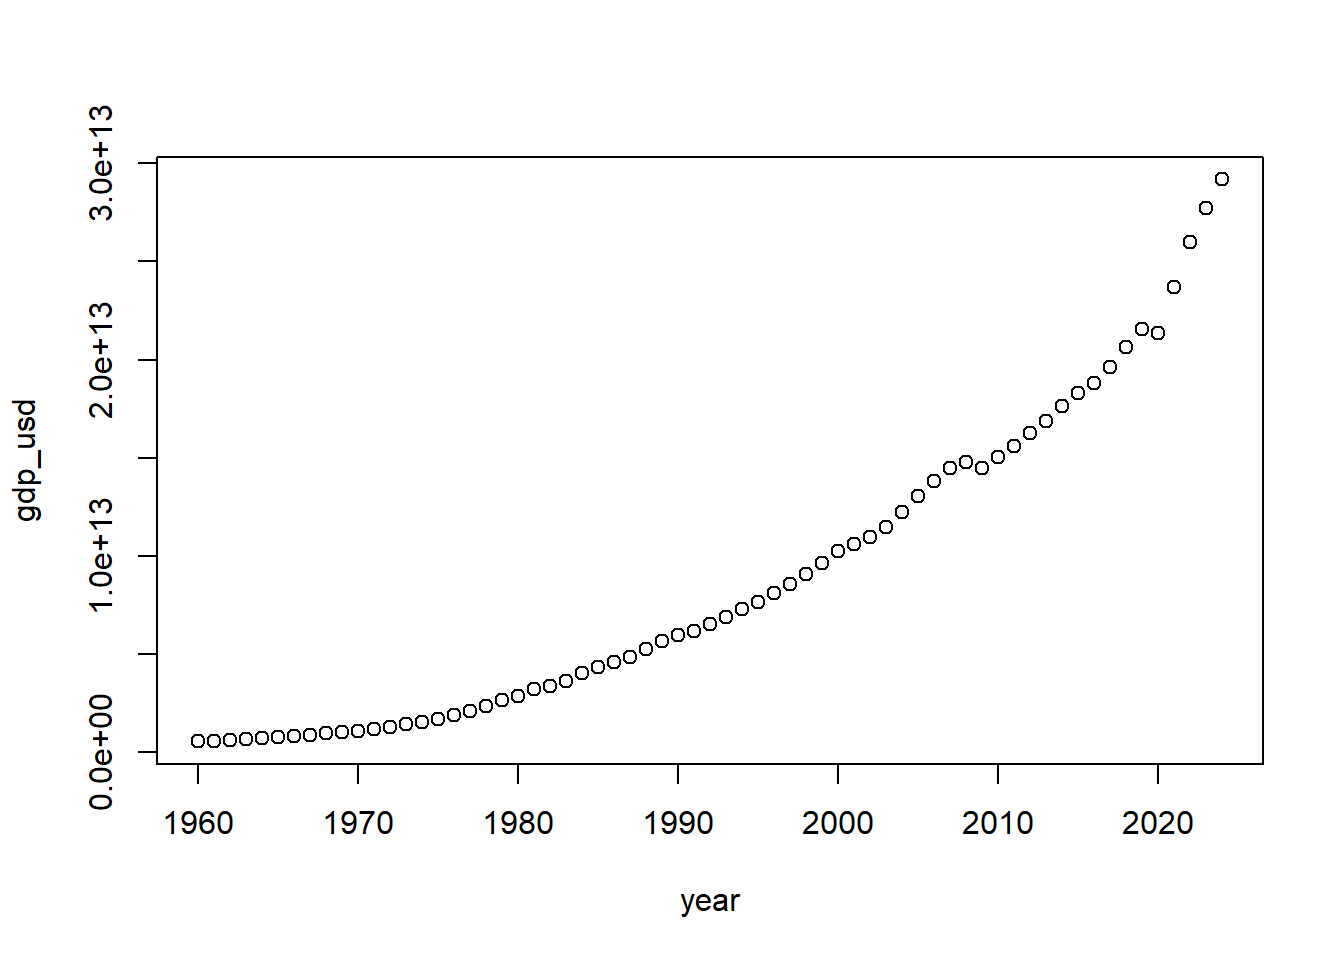
\includegraphics[keepaspectratio]{Lecture-4_files/figure-pdf/unnamed-chunk-10-1.pdf}}

\bookmarksetup{startatroot}

\chapter{HTML Data}\label{html-data}

So far this semester we have investigated how we can scrape both JSON
and XML data from webpages. Another method we will investigate is HTML
scraping. This will be a useful topic considering every webpage is
written in HTML with the content wrapped in tags (like
\textless h1\textgreater{} for titles, \textless p\textgreater{} for
paragraphs, and \textless table\textgreater{} for tables, and many many
more). Within these tags we can have attributes, just like we did with
XML data, that will make it easier to target specific content. Before we
dive into the material, a helpful hint in determining which tags and
attributes to reference it to right-click on the text in the browser and
choosing ``Inspect''. This will allow us to view the raw HTML structure,
which we can use to identify what tag is related to the content, and
then we can extract it using the \texttt{revest} library in R.

\section{Introductory Example}\label{introductory-example}

To understand the general idea of this, we will look at the website
\url{https://example.com/}. If we were to right-click on the page and
``View Page Source'', it will open up another tab to show us the raw
HTML structure. Scrolling to the very bottom of the page, we can see the
\textless body\textgreater{} tag, which displays the text currently on
the page. It should look something like this:

\begin{Shaded}
\begin{Highlighting}[]
\NormalTok{\textless{}body\textgreater{}}
\NormalTok{\textless{}div\textgreater{}}
\NormalTok{    \textless{}h1\textgreater{}Example Domain\textless{}/h1\textgreater{}}
\NormalTok{    \textless{}p\textgreater{}This domain is for use in illustrative examples in documents. You may use this}
\NormalTok{    domain in literature without prior coordination or asking for permission.\textless{}/p\textgreater{}}
\NormalTok{    \textless{}p\textgreater{}\textless{}a href="https://www.iana.org/domains/example"\textgreater{}More information...\textless{}/a\textgreater{}\textless{}/p\textgreater{}}
\NormalTok{\textless{}/div\textgreater{}}
\NormalTok{\textless{}/body\textgreater{}}
\NormalTok{\textless{}/html\textgreater{}}
\end{Highlighting}
\end{Shaded}

In order to extract this data and use in R, we can use the
\texttt{rvest} library along with the \texttt{read\_html()},
\texttt{html\_elements()}, and \texttt{html\_text()} functions. In the
example below, we can see how we pull the main heading information
stored in the \textless h1\textgreater{} tag.

\begin{Shaded}
\begin{Highlighting}[]
\FunctionTok{library}\NormalTok{(rvest)}
\FunctionTok{library}\NormalTok{(dplyr)}

\NormalTok{page }\OtherTok{\textless{}{-}} \FunctionTok{read\_html}\NormalTok{(}\StringTok{"https://example.com"}\NormalTok{)}
\NormalTok{page }\SpecialCharTok{|\textgreater{}} \FunctionTok{html\_elements}\NormalTok{(}\StringTok{"h1"}\NormalTok{) }\SpecialCharTok{|\textgreater{}} \FunctionTok{html\_text}\NormalTok{()}
\end{Highlighting}
\end{Shaded}

\begin{verbatim}
[1] "Example Domain"
\end{verbatim}

We can also extract the paragraph text stored in the
\textless p\textgreater{} tag. Notice how we get multiple character
elements because there are multiple \textless p\textgreater{} tags
present.

\begin{Shaded}
\begin{Highlighting}[]
\NormalTok{page }\SpecialCharTok{|\textgreater{}} \FunctionTok{html\_elements}\NormalTok{(}\StringTok{"p"}\NormalTok{) }\SpecialCharTok{|\textgreater{}} \FunctionTok{html\_text}\NormalTok{()}
\end{Highlighting}
\end{Shaded}

\begin{verbatim}
[1] "This domain is for use in illustrative examples in documents. You may use this\n    domain in literature without prior coordination or asking for permission."
[2] "More information..."                                                                                                                                          
\end{verbatim}

If we wanted to only extract certain

tags, we could use a few different methods. If we only wanted the first
one we could alter the function to be \texttt{html\_element()}. We could
also use the \texttt{nth-of-type()} argument to select which one to
extract. Finally, if the tag has a nested element, we can reference it
by typing in both tags as seen below:

\begin{Shaded}
\begin{Highlighting}[]
\NormalTok{page }\SpecialCharTok{|\textgreater{}} \FunctionTok{html\_element}\NormalTok{(}\StringTok{"p"}\NormalTok{) }\SpecialCharTok{|\textgreater{}} \FunctionTok{html\_text}\NormalTok{()}
\end{Highlighting}
\end{Shaded}

\begin{verbatim}
[1] "This domain is for use in illustrative examples in documents. You may use this\n    domain in literature without prior coordination or asking for permission."
\end{verbatim}

\begin{Shaded}
\begin{Highlighting}[]
\NormalTok{page }\SpecialCharTok{|\textgreater{}} \FunctionTok{html\_elements}\NormalTok{(}\StringTok{"p:nth{-}of{-}type(1)"}\NormalTok{) }\SpecialCharTok{|\textgreater{}} \FunctionTok{html\_text}\NormalTok{()}
\end{Highlighting}
\end{Shaded}

\begin{verbatim}
[1] "This domain is for use in illustrative examples in documents. You may use this\n    domain in literature without prior coordination or asking for permission."
\end{verbatim}

\begin{Shaded}
\begin{Highlighting}[]
\NormalTok{page }\SpecialCharTok{|\textgreater{}} \FunctionTok{html\_elements}\NormalTok{(}\StringTok{"p:nth{-}of{-}type(2)"}\NormalTok{) }\SpecialCharTok{|\textgreater{}} \FunctionTok{html\_text}\NormalTok{()}
\end{Highlighting}
\end{Shaded}

\begin{verbatim}
[1] "More information..."
\end{verbatim}

\begin{Shaded}
\begin{Highlighting}[]
\NormalTok{page }\SpecialCharTok{|\textgreater{}} \FunctionTok{html\_elements}\NormalTok{(}\StringTok{"p a"}\NormalTok{) }\SpecialCharTok{|\textgreater{}} \FunctionTok{html\_text}\NormalTok{()}
\end{Highlighting}
\end{Shaded}

\begin{verbatim}
[1] "More information..."
\end{verbatim}

In order to access the attribute of the tag, we can use the
\texttt{html\_attr()} function as seen below:

\begin{Shaded}
\begin{Highlighting}[]
\NormalTok{page }\SpecialCharTok{|\textgreater{}} \FunctionTok{html\_element}\NormalTok{(}\StringTok{"p a"}\NormalTok{) }\SpecialCharTok{|\textgreater{}} \FunctionTok{html\_attr}\NormalTok{(}\StringTok{"href"}\NormalTok{)}
\end{Highlighting}
\end{Shaded}

\begin{verbatim}
[1] "https://www.iana.org/domains/example"
\end{verbatim}

\section{BBC Example}\label{bbc-example}

Now that we have seen a basic example, lets see a slightly more complex
one. If we go to \url{https://www.bbc.com/news}, we can see a lot of
different news articles along with short descriptions of them. Looking
at the ``View Page Source'', we can see that it is virtually unreadable
due to the vast amount of data present. And since it will not be fun to
read through it all to see what the different tags are called, we can
right-click the text we are interested in and then ``Inspect'' it. A
pane will appear on half of the screen that allows us to see what tag
the data is saved under. In the example below, we can see the article
title is saved under the \textless h2\textgreater{} tag.

\begin{center}
\pandocbounded{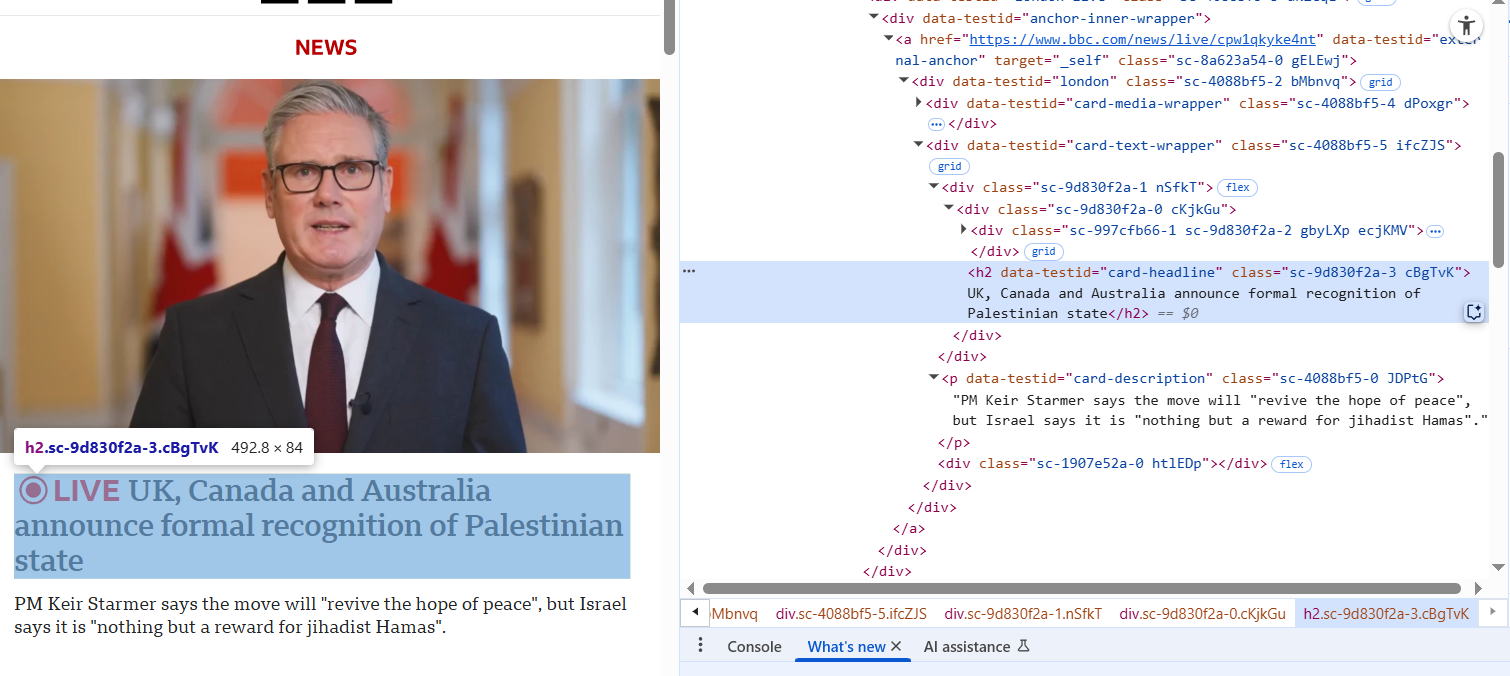
\includegraphics[keepaspectratio]{Images/BBC-Example-Headers.PNG}}
\end{center}
Looking at the description, we can see that it is saved under the
\textless p\textgreater{} tag.

\begin{center}
\pandocbounded{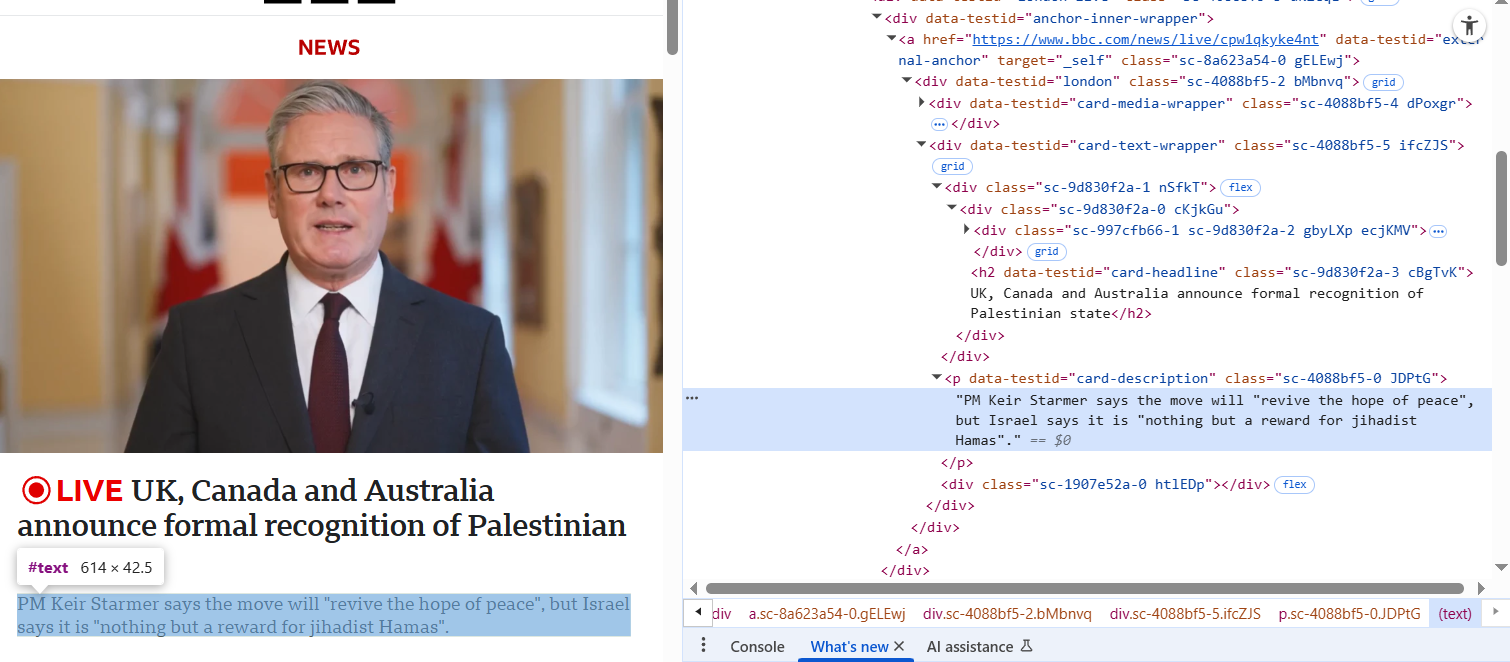
\includegraphics[keepaspectratio]{Images/BBC-Example-Description.PNG}}
\end{center}

We can this use this information to scrape the webpage and to get the
article titles and descriptions in a similar manner to what we did
before

\begin{Shaded}
\begin{Highlighting}[]
\CommentTok{\# Note: when you run this you might get different results as the webpage is constantly updated}

\NormalTok{bbc }\OtherTok{\textless{}{-}} \FunctionTok{read\_html}\NormalTok{(}\StringTok{"https://www.bbc.com"}\NormalTok{)}

\NormalTok{bbc }\SpecialCharTok{|\textgreater{}} \FunctionTok{html\_elements}\NormalTok{(}\StringTok{"h2"}\NormalTok{) }\SpecialCharTok{|\textgreater{}} \FunctionTok{html\_text}\NormalTok{() }\SpecialCharTok{|\textgreater{}} \FunctionTok{head}\NormalTok{()}
\end{Highlighting}
\end{Shaded}

\begin{verbatim}
[1] "Recognising Palestinian statehood opens another question - who would lead it?"
[2] "UK rewarding Hamas, says mother of freed British-Israeli hostage"             
[3] "Recognising Palestinian statehood opens another question - who would lead it?"
[4] "UK rewarding Hamas, says mother of freed British-Israeli hostage"             
[5] "UK formally recognises Palestinian state"                                     
[6] "Trump arrives at Charlie Kirk memorial as tens of thousands attend service"   
\end{verbatim}

\begin{Shaded}
\begin{Highlighting}[]
\NormalTok{bbc }\SpecialCharTok{|\textgreater{}} \FunctionTok{html\_elements}\NormalTok{(}\StringTok{"p"}\NormalTok{) }\SpecialCharTok{|\textgreater{}} \FunctionTok{html\_text}\NormalTok{(}\AttributeTok{trim=}\ConstantTok{TRUE}\NormalTok{) }\SpecialCharTok{|\textgreater{}} \FunctionTok{head}\NormalTok{()}
\end{Highlighting}
\end{Shaded}

\begin{verbatim}
[1] "With the president approaching 90 years of age and another possible candidate in jail, finding the right leadership would be a challenge"             
[2] "Sir Keir Starmer has insisted Hamas can have \"no future, no role in government, no role in security\"."                                              
[3] "With the president approaching 90 years of age and another possible candidate in jail, finding the right leadership would be a challenge"             
[4] "Sir Keir Starmer has insisted Hamas can have \"no future, no role in government, no role in security\"."                                              
[5] "Canada and Australia also announced the move on Sunday, with Israeli PM Benjamin Netanyahu accusing leaders of giving a \"huge reward to terrorism\"."
[6] "The conservative activist was shot and killed while speaking to students at a university in Utah on 10 September."                                    
\end{verbatim}

We could do something similar and get the contents of the article as
well. We should be weary to do this though, as this information is
copyrighted by the BBC and thus we should respect their work product.
For this example, we will just display the first few sentences as an
example:

\begin{Shaded}
\begin{Highlighting}[]
\NormalTok{article }\OtherTok{\textless{}{-}} \FunctionTok{read\_html}\NormalTok{(}\StringTok{"https://www.bbc.com/news/articles/ce800enrglzo"}\NormalTok{)}

\NormalTok{article }\SpecialCharTok{|\textgreater{}} \FunctionTok{html\_elements}\NormalTok{(}\StringTok{"p"}\NormalTok{) }\SpecialCharTok{|\textgreater{}} \FunctionTok{html\_text}\NormalTok{() }\SpecialCharTok{|\textgreater{}} \FunctionTok{head}\NormalTok{(}\DecValTok{4}\NormalTok{)}
\end{Highlighting}
\end{Shaded}

\begin{verbatim}
[1] "Sir Keir Starmer has announced the UK's recognition of a Palestinian state, in what represents a significant change in government policy."                                                                                                   
[2] "In a video statement on X, the prime minister said: \"In the face of the growing horror in the Middle East we are acting to keep alive the possibility of peace and a two-state solution.\""                                                 
[3] "Australia and Canada also announced formal recognition of the state of Palestine, with Portugal and France expected to follow."                                                                                                              
[4] "The decision has drawn fierce criticism from the Israeli government, families of hostages held in Gaza and some Conservatives. Responding on Sunday, Israeli Prime Minister Benjamin Netanyahu said a Palestinian state \"will not happen\"."
\end{verbatim}

\section{Scraping Tables}\label{scraping-tables}

The last example we will look at for now is scraping an HTML table from
a webpage and making it available to us in R. For this example, we will
look at the Mount St.~Mary's Basketball Teams statistics:
\url{https://mountathletics.com/sports/mens-basketball/stats/2024-25}.
We can see that there are a number of different tables on the page, and
by right-clicking the table and hitting the ``Inspect'' button, we can
see that they are all saved under the \textless table\textgreater{} tag.
We can screpe it in a similar manner, only this time we will need to use
the \texttt{html\_table()} function.

\begin{Shaded}
\begin{Highlighting}[]
\NormalTok{mount }\OtherTok{\textless{}{-}} \FunctionTok{read\_html}\NormalTok{(}\StringTok{"https://mountathletics.com/sports/mens{-}basketball/stats/2024{-}25"}\NormalTok{)}

\NormalTok{basketball\_tables }\OtherTok{\textless{}{-}}\NormalTok{ mount }\SpecialCharTok{|\textgreater{}} \FunctionTok{html\_elements}\NormalTok{(}\StringTok{"table"}\NormalTok{) }\SpecialCharTok{|\textgreater{}} \FunctionTok{html\_table}\NormalTok{(}\AttributeTok{fill =} \ConstantTok{TRUE}\NormalTok{) }

\NormalTok{overall\_stats }\OtherTok{\textless{}{-}}\NormalTok{ basketball\_tables[[}\DecValTok{2}\NormalTok{]]}

\NormalTok{overall\_stats}
\end{Highlighting}
\end{Shaded}

\begin{verbatim}
# A tibble: 18 x 27
   `#`   Player  GP    GS    Minutes Minutes FG    FG    FG    `3PT` `3PT` `3PT`
   <chr> <chr>   <chr> <chr> <chr>   <chr>   <chr> <chr> <chr> <chr> <chr> <chr>
 1 "#"   "Playe~ GP    "GS"  TOT     AVG     FGM   FGA   FG%   3PT   3PTA  3PT% 
 2 "04"  "Adeba~ 36    "36"  1043    29.0    175   340   .515  22    72    .306 
 3 "08"  "Hobbs~ 30    "26"  839     28.0    123   333   .369  54    173   .312 
 4 "13"  "Ard J~ 21    "3"   512     24.4    87    163   .534  1     6     .167 
 5 "14"  "Cordi~ 35    "33"  1037    29.6    160   269   .595  2     7     .286 
 6 "01"  "Pache~ 30    "30"  846     28.2    88    188   .468  77    166   .464 
 7 "45"  "Lipsc~ 36    "36"  1209    33.6    67    190   .353  36    106   .340 
 8 "02"  "Keyes~ 32    "2"   616     19.3    71    190   .374  48    133   .361 
 9 "23"  "Ervin~ 34    "14"  525     15.4    60    169   .355  14    52    .269 
10 "09"  "Khadr~ 29    "0"   322     11.1    26    84    .310  12    51    .235 
11 "10"  "Haigh~ 19    "0"   123     6.5     12    45    .267  10    41    .244 
12 "05"  "Dread~ 18    "0"   120     6.7     12    25    .480  7     14    .500 
13 "03"  "Ogunf~ 3     "0"   8       2.7     2     2     1.000 0     0     .000 
14 "12"  "Wilso~ 24    "0"   96      4.0     6     16    .375  2     6     .333 
15 "06"  "Hartm~ 2     "0"   4       2.0     0     0     .000  0     0     .000 
16 "TM"  "Team\~ 36    "0"   0       0.0     0     0     .000  0     0     .000 
17 ""    "Total" 36    ""    7300    202.8   889   2014  .441  285   827   .345 
18 ""    "Oppon~ 36    ""    7300    202.8   903   2196  .411  313   989   .316 
# i 15 more variables: FT <chr>, FT <chr>, FT <chr>, Scoring <chr>,
#   Scoring <chr>, Rebounds <chr>, Rebounds <chr>, Rebounds <chr>,
#   Rebounds <chr>, PF <chr>, AST <chr>, TO <chr>, STL <chr>, BLK <chr>,
#   `Bio Link` <chr>
\end{verbatim}

The table we scraped off of the website has 2 different header rows, one
being more categorical (``minutes'', ``fg'', ``scoring'', etc.) with the
sub-header row being more detailed. We can combine the header names so
that ``Minutes\_AVG'', ``Scoring\_AVG'', and ``Rebounds\_AVG'' are not
confused for each other. We would want to go ahead and clean the other
column names up as well, as ``GS\_GS'' is redundant, but we will let
that be an exercise for the reader. One last thing we will do it see how
we can convert all of the columns except for name and jersey number into
a numeric value using the \texttt{mutate()} and \texttt{across()}
functions.

\begin{Shaded}
\begin{Highlighting}[]
\FunctionTok{colnames}\NormalTok{(overall\_stats) }\OtherTok{\textless{}{-}} \FunctionTok{paste}\NormalTok{(}\FunctionTok{colnames}\NormalTok{(overall\_stats), overall\_stats[}\DecValTok{1}\NormalTok{, ], }\AttributeTok{sep =} \StringTok{"\_"}\NormalTok{)}

\NormalTok{overall\_stats }\OtherTok{\textless{}{-}}\NormalTok{ overall\_stats[}\SpecialCharTok{{-}}\DecValTok{1}\NormalTok{,]}

\NormalTok{overall\_stats\_clean }\OtherTok{\textless{}{-}}\NormalTok{ overall\_stats }\SpecialCharTok{|\textgreater{}} 
  \FunctionTok{mutate}\NormalTok{( }\FunctionTok{across}\NormalTok{(}\SpecialCharTok{{-}}\FunctionTok{c}\NormalTok{(Player\_Player, }\StringTok{\textasciigrave{}}\AttributeTok{\#\_\#}\StringTok{\textasciigrave{}}\NormalTok{), }\SpecialCharTok{\textasciitilde{}} \FunctionTok{as.numeric}\NormalTok{(.) ))}
\end{Highlighting}
\end{Shaded}

\begin{verbatim}
Warning: There was 1 warning in `mutate()`.
i In argument: `across(-c(Player_Player, `#_#`), ~as.numeric(.))`.
Caused by warning:
! NAs introduced by coercion
\end{verbatim}

\begin{Shaded}
\begin{Highlighting}[]
\NormalTok{overall\_stats\_clean}
\end{Highlighting}
\end{Shaded}

\begin{verbatim}
# A tibble: 17 x 27
   `#_#` Player_Player         GP_GP GS_GS Minutes_TOT Minutes_AVG FG_FGM FG_FGA
   <chr> <chr>                 <dbl> <dbl>       <dbl>       <dbl>  <dbl>  <dbl>
 1 "04"  "Adebayo, Dola\r\n  ~    36    36        1043        29      175    340
 2 "08"  "Hobbs, Dallas\r\n  ~    30    26         839        28      123    333
 3 "13"  "Ard Jr., Terrell\r\~    21     3         512        24.4     87    163
 4 "14"  "Cordilia, Jedy\r\n ~    35    33        1037        29.6    160    269
 5 "01"  "Pacheco, Carmelo\r\~    30    30         846        28.2     88    188
 6 "45"  "Lipscomb, Xavier\r\~    36    36        1209        33.6     67    190
 7 "02"  "Keyes, Arlandus\r\n~    32     2         616        19.3     71    190
 8 "23"  "Ervin, Javon\r\n   ~    34    14         525        15.4     60    169
 9 "09"  "Khadre Kébé, Abdou\~    29     0         322        11.1     26     84
10 "10"  "Haigh, Patrick\r\n ~    19     0         123         6.5     12     45
11 "05"  "Dread, Malcolm\r\n ~    18     0         120         6.7     12     25
12 "03"  "Ogunfuye, Jonathan\~     3     0           8         2.7      2      2
13 "12"  "Wilson, Trey\r\n   ~    24     0          96         4        6     16
14 "06"  "Hartman, Jaxon\r\n ~     2     0           4         2        0      0
15 "TM"  "Team\r\n           ~    36     0           0         0        0      0
16 ""    "Total"                  36    NA        7300       203.     889   2014
17 ""    "Opponents"              36    NA        7300       203.     903   2196
# i 19 more variables: `FG_FG%` <dbl>, `3PT_3PT` <dbl>, `3PT_3PTA` <dbl>,
#   `3PT_3PT%` <dbl>, FT_FTM <dbl>, FT_FTA <dbl>, `FT_FT%` <dbl>,
#   Scoring_PTS <dbl>, Scoring_AVG <dbl>, Rebounds_OFF <dbl>,
#   Rebounds_DEF <dbl>, Rebounds_TOT <dbl>, Rebounds_AVG <dbl>, PF_PF <dbl>,
#   AST_AST <dbl>, TO_TO <dbl>, STL_STL <dbl>, BLK_BLK <dbl>,
#   `Bio Link_Bio Link` <dbl>
\end{verbatim}




\end{document}
